\documentclass{article}\usepackage[]{graphicx}\usepackage[svgnames]{xcolor}
% maxwidth is the original width if it is less than linewidth
% otherwise use linewidth (to make sure the graphics do not exceed the margin)
\makeatletter
\def\maxwidth{ %
  \ifdim\Gin@nat@width>\linewidth
    \linewidth
  \else
    \Gin@nat@width
  \fi
}
\makeatother

\definecolor{fgcolor}{rgb}{0.345, 0.345, 0.345}
\newcommand{\hlnum}[1]{\textcolor[rgb]{0.686,0.059,0.569}{#1}}%
\newcommand{\hlstr}[1]{\textcolor[rgb]{0.192,0.494,0.8}{#1}}%
\newcommand{\hlcom}[1]{\textcolor[rgb]{0.678,0.584,0.686}{\textit{#1}}}%
\newcommand{\hlopt}[1]{\textcolor[rgb]{0,0,0}{#1}}%
\newcommand{\hlstd}[1]{\textcolor[rgb]{0.345,0.345,0.345}{#1}}%
\newcommand{\hlkwa}[1]{\textcolor[rgb]{0.161,0.373,0.58}{\textbf{#1}}}%
\newcommand{\hlkwb}[1]{\textcolor[rgb]{0.69,0.353,0.396}{#1}}%
\newcommand{\hlkwc}[1]{\textcolor[rgb]{0.333,0.667,0.333}{#1}}%
\newcommand{\hlkwd}[1]{\textcolor[rgb]{0.737,0.353,0.396}{\textbf{#1}}}%
\let\hlipl\hlkwb

\usepackage{framed}
\makeatletter
\newenvironment{kframe}{%
 \def\at@end@of@kframe{}%
 \ifinner\ifhmode%
  \def\at@end@of@kframe{\end{minipage}}%
  \begin{minipage}{\columnwidth}%
 \fi\fi%
 \def\FrameCommand##1{\hskip\@totalleftmargin \hskip-\fboxsep
 \colorbox{shadecolor}{##1}\hskip-\fboxsep
     % There is no \\@totalrightmargin, so:
     \hskip-\linewidth \hskip-\@totalleftmargin \hskip\columnwidth}%
 \MakeFramed {\advance\hsize-\width
   \@totalleftmargin\z@ \linewidth\hsize
   \@setminipage}}%
 {\par\unskip\endMakeFramed%
 \at@end@of@kframe}
\makeatother

\definecolor{shadecolor}{rgb}{.97, .97, .97}
\definecolor{messagecolor}{rgb}{0, 0, 0}
\definecolor{warningcolor}{rgb}{1, 0, 1}
\definecolor{errorcolor}{rgb}{1, 0, 0}
\newenvironment{knitrout}{}{} % an empty environment to be redefined in TeX

\usepackage{alltt}
\usepackage[svgnames]{xcolor}
\usepackage[british]{babel}
\usepackage[protrusion,expansion,tracking,kerning,babel,final]{microtype}
\usepackage[margin=1in]{geometry}
\usepackage[pdfversion=1.7]{hyperref}
\usepackage[shortlabels]{enumitem}
\usepackage{graphicx}
\usepackage{mathtools}
\usepackage{cleveref}
\usepackage{booktabs}
\usepackage{nicematrix}
\usepackage{derivative}
\usepackage{etoolbox}
\usepackage{siunitx}
\usepackage{listings}
\usepackage{tikz}
\newcommand*\circled[1]{\tikz[baseline=(char.base)]{\node[shape=circle,draw,inner sep=2pt] (char) {#1};}}
\usepackage{bm}
\usepackage[T1]{fontenc}
\makeatletter
\renewcommand\subsection{\@startsection{subsection}{2}{\z@}%
                                     {-3.25ex\@plus -1ex \@minus -.2ex}%
                                     {1.5ex \@plus .2ex}%
                                     {\normalfont\large\bfseries\scshape\color{Blue}}}
\makeatother

\lstset{frame=none,
  language=R,
  showstringspaces=false,
  columns=flexible,
  numbers=none,
  basicstyle={\small\ttfamily},
  keywordstyle=\color{Blue},
  stringstyle=\color{Red},
  commentstyle=\color{DarkGreen},
  breaklines=true,
  breakatwhitespace=true,
  moredelim=**[is][\color{blue}]{@}{@},
  tabsize=3}


% Functions
\providecommand\given{} % just to make sure it exists
\DeclarePairedDelimiterXPP{\E}[1]{\operatorname{\text{E}}}[]{}{%
    \renewcommand\given{\nonscript\:\delimsize\vert\nonscript\:\mathopen{}}%
    \ifblank{#1}{\:\cdot\:}%
    #1}%
\DeclarePairedDelimiterXPP{\V}[1]{\operatorname{\Field{V}}}(){}{%
    \renewcommand\given{\nonscript\:\delimsize\vert\nonscript\:\mathopen{}}%
    \ifblank{#1}{\:\cdot\:}%
    #1}%
\DeclarePairedDelimiterXPP{\Var}[1]{\operatorname{\text{Var}}}(){}{%
    \renewcommand\given{\nonscript\:\delimsize\vert\nonscript\:\mathopen{}}%
    \ifblank{#1}{\:\cdot\:}%
    #1}%
\DeclarePairedDelimiterXPP{\Cov}[1]{\operatorname{\text{Cov}}}(){}{%
    \renewcommand\given{\nonscript\:\delimsize\vert\nonscript\:\mathopen{}}%
    \ifblank{#1}{\:\cdot\:}%
    #1}%
\DeclarePairedDelimiterXPP\Prob[1]{\operatorname{\Field{P}}}(){}{%
    \renewcommand\given{\nonscript\:\delimsize\vert\nonscript\:\mathopen{}}%
    \ifblank{#1}{\:\cdot\:}%
    #1}%
\DeclarePairedDelimiterXPP\Ind[1]{\operatorname{\Field{I}}}\{\}{}{%
    \renewcommand\given{\nonscript\:\delimsize\vert\nonscript\:\mathopen{}}%
    \ifblank{#1}{\:\cdot\:}%
    #1}%
\DeclarePairedDelimiterXPP{\se}[1]{\operatorname{\text{se}}}(){}{%
    \ifblank{#1}{\:\cdot\:}%
    #1}%
\DeclarePairedDelimiterXPP{\estse}[1]{\widehat{\operatorname{\text{se}}}}(){}{%
    \ifblank{#1}{\:\cdot\:}%
    #1}%
\DeclarePairedDelimiterXPP{\estV}[1]{\widehat{\operatorname{\Field{V}}}}(){}{
    \renewcommand\given{\nonscript\:\delimsize\vert\nonscript\:\mathopen{}}%
    \ifblank{#1}{\:\cdot\:}%
    #1}%
\DeclarePairedDelimiterXPP{\estVar}[1]{\widehat{\operatorname{\text{Var}}}}(){}{
    \renewcommand\given{\nonscript\:\delimsize\vert\nonscript\:\mathopen{}}%
    \ifblank{#1}{\:\cdot\:}%
    #1}%
\let\exp\relax%
\let\log\relax%
\let\ln\relax%
\DeclarePairedDelimiterXPP{\exp}[1]{\operatorname{\text{exp}}}\{\}{}{#1}%
\DeclarePairedDelimiterXPP{\log}[1]{\operatorname{\text{log}}}(){}{#1}%
\DeclarePairedDelimiterXPP{\ln}[1]{\operatorname{\text{ln}}}(){}{#1}%
\DeclarePairedDelimiterXPP{\diag}[1]{\operatorname{\text{diag}}}(){}{#1}%
\DeclarePairedDelimiterXPP{\sign}[1]{\operatorname{\text{sign}}}(){}{#1}%

\DeclarePairedDelimiterXPP{\expit}[1]{\operatorname{\text{expit}}}(){}{#1}%
\DeclarePairedDelimiterXPP{\logit}[1]{\operatorname{\text{logit}}}(){}{#1}%
\newcommand{\HN}{\text{H}_0}%
\newcommand{\HA}{\text{H}_{\text{A}}}%

% Distributions
\DeclarePairedDelimiterXPP{\N}[1]{\mathcal{N}}(){}{#1}%
\DeclarePairedDelimiterXPP{\Poisson}[1]{\text{Poisson}}(){}{#1}%
\DeclarePairedDelimiterXPP{\Bin}[1]{\text{Bin}}(){}{#1}%
\DeclarePairedDelimiterXPP{\Binomial}[1]{\text{Binomial}}(){}{#1}%
\DeclarePairedDelimiterXPP{\Bernoulli}[1]{\text{Bernoulli}}(){}{#1}%
\DeclarePairedDelimiterXPP{\MVN}[1]{\text{MVN}}(){}{#1}%

\newcommand{\iid}{\overset{\text{iid}}{\sim}}%
\newcommand{\ind}{\overset{\text{ind}}{\sim}}%
\newcommand{\OR}{\text{OR}}%
\newcommand{\RR}{\text{RR}}%

\DeclarePairedDelimiter\abs{\lvert}{\rvert}
% can be useful to refer to this outside \Set
\newcommand\SetSymbol[1][]{%
    \nonscript\:#1\vert{}
    \allowbreak\nonscript\:
    \mathopen{}}
\DeclarePairedDelimiterX\Set[1]\{\}{%
    \renewcommand\given{:}
    #1
}
\DeclareMathOperator*{\argmax}{arg\,max}
\DeclareMathOperator*{\argmin}{arg\,min}
\DeclareMathOperator*{\arginf}{arg\,inf}
\DeclareMathOperator*{\argsup}{arg\,sup}

% Table of Contents
\hypersetup{colorlinks,linkcolor=[rgb]{0,0.5,1}}%

\title{%
    {\LARGE Generalized Linear Models}\\%
    {\large STAT 431/STAT 831}\\%
    {\normalsize Spring 2022 (idk)}%
}%
\author{%
    \LaTeX{}er: \emph{Cameron Roopnarine}\\%
    Instructor: \emph{Leilei Zeng}%
}%
\date{\today}%

\providecommand{\RandomVector}[1]{\bm{#1}}% general vectors in bold italic
\providecommand{\Vector}[1]{\bm{#1}}% general vectors in bold italic
\providecommand{\Matrix}[1]{\bm{#1}}
\providecommand{\MatrixCal}[1]{\bm{\mathcal{#1}}}
\providecommand{\Field}[1]{\bm{#1}}

\usepackage{stackengine}
\usepackage[british]{isodate}
\newcommand{\makeheading}[2]%
{%
\begin{center}%
    \makebox[\linewidth]{\raisebox{-.5ex}[0cm][0cm]{\stackanchor{\textcolor{Gray}{\textsc{#1}}}{\scriptsize\itshape\printyearoff #2}\;}\color{Crimson!50}\hrulefill}%
\end{center}%
}%

\usepackage[breakable]{tcolorbox}
\tcbset{
    regular/.style={
        boxrule=0pt,
        breakable,
        sharp corners,
    }
}

\newtcolorbox{Example}[1]{regular,colframe=Green!20!white,colback=Green!10!white,coltitle=Green,title={#1}}%
\newtcolorbox{Regular}[1]{regular,colframe=Navy!15!white,colback=Navy!5!white,coltitle=Navy,title={#1}}%
\newtcolorbox{Result}[1]{regular,colframe=Red!15!white,colback=Red!5!white,coltitle=Red,title={#1}}%

\hypersetup{colorlinks=true,%
linkcolor=[rgb]{0,0.5,1},%
pdftitle={Generalized Linear Models and their Applications (STAT 431/STAT 831)},%
pdfauthor={Cameron Roopnarine, Leilei Zeng},%
pdfsubject={Statistics},%
pdfkeywords={University of Waterloo, Fall 2021 (1219)}}%

\title{%
\LARGE Generalized Linear Models and their Applications\\%
\large STAT 431/STAT 831\thanks{STAT 431 $ \equiv $ STAT 831}\\%
\normalsize Fall 2021 (1219)\thanks{Online Course}}%
\author{Cameron Roopnarine\thanks{\LaTeX{}er}\and Leilei Zeng\thanks{Instructor}}%
\date{\today}%

\IfFileExists{upquote.sty}{\usepackage{upquote}}{}
\begin{document}


\maketitle
\newpage
\tableofcontents
\newpage

\makeheading{Week 1}{\daterange{2021-09-08}{2021-09-10}}
\section*{Topic 1a: Review of Linear Regression}
\addcontentsline{toc}{section}{Topic 1a: Review of Linear Regression}

\subsection*{Example: low birthweight infants study\footnote{Principles of Biostatistics 2nd Edition by Marcello Pagano, Kimberlee Gauvreau.}}
A study was conducted at two teaching
hospitals in Boston, Massachusetts,
where the head circumference, gestational age and some other variables
are recorded for 100 low birth weight
infants.

Question: what is the relationship between \textcolor{Blue}{\emph{gestational age}} \& \textcolor{Blue}{head circumference}?
% \begin{noindent}
\begin{knitrout}
\definecolor{shadecolor}{rgb}{0.969, 0.969, 0.969}\color{fgcolor}

{\centering 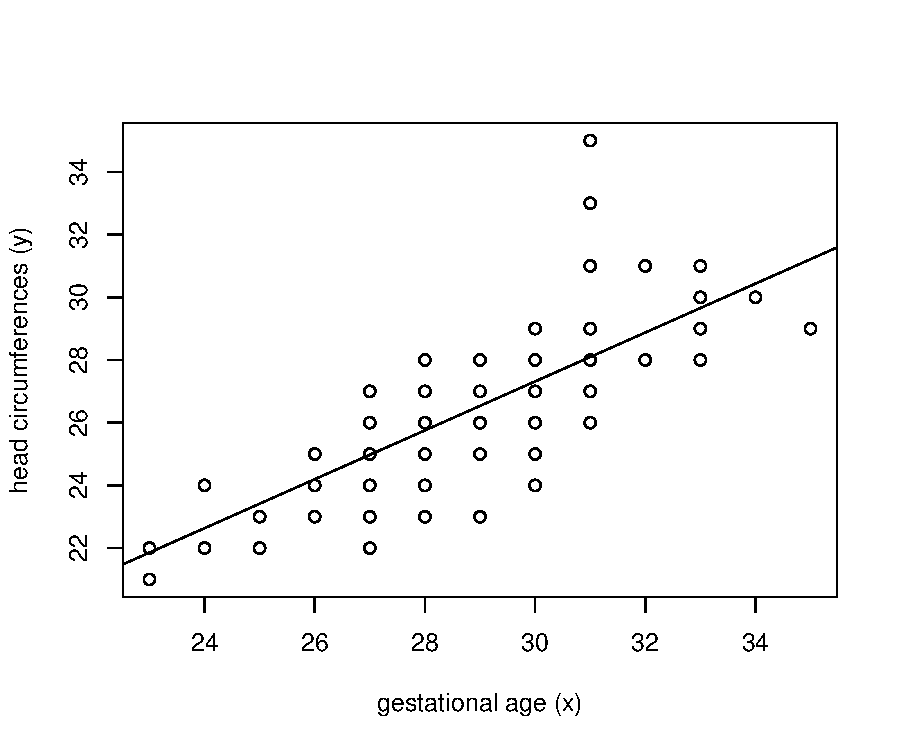
\includegraphics[width=\maxwidth]{figure/unnamed-chunk-8-1} 

}


\end{knitrout}
% \end{noindent}
We wish to model the relationship between \emph{gestational age} and \emph{head
    circumference} using a straight line!
% \begin{noidnent}
\begin{knitrout}
\definecolor{shadecolor}{rgb}{0.969, 0.969, 0.969}\color{fgcolor}

{\centering 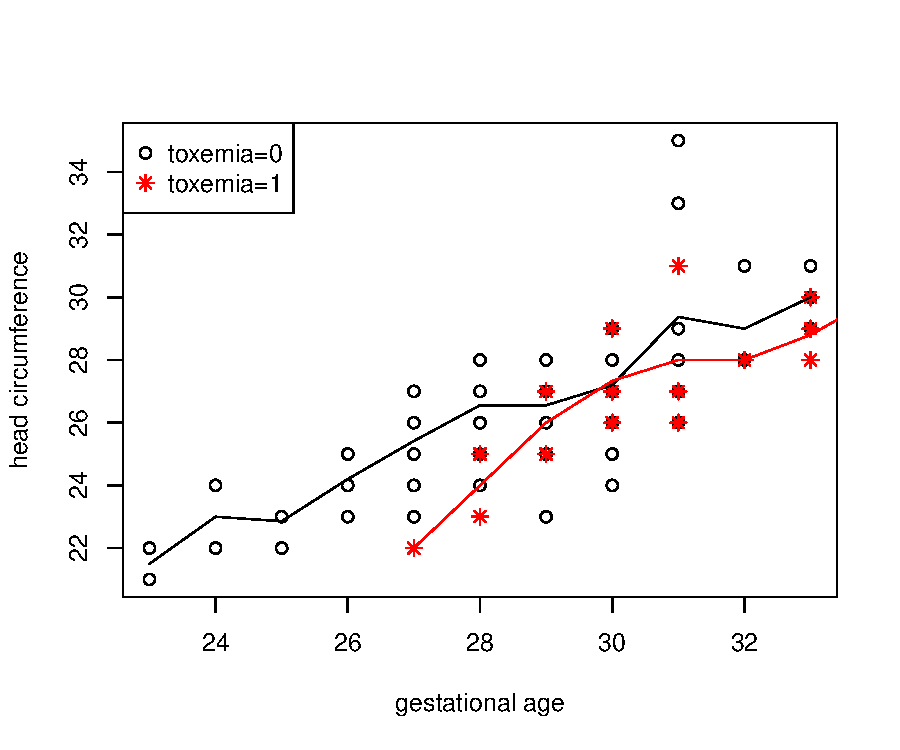
\includegraphics[width=\maxwidth]{figure/unnamed-chunk-9-1} 

}


\end{knitrout}
% \end{noidnent}

\subsection*{The Model Fitting Process}
\begin{enumerate}[label=\color{Blue}\protect\circled{\arabic*}]
    \item \textcolor{Red}{Model Specification}: select a probability distribution for the response
          variable and a linear equation linking the response to the explanatory
          variables.
    \item \textcolor{Red}{Estimation}: finding the equation (the parameters of the model).
    \item \textcolor{Red}{Model checking}: how well does the model fit the data?
    \item \textcolor{Red}{Inference}: interpret the fitted model, calculate confidence intervals,
          conduct hypothesis tests.
\end{enumerate}

\subsection*{\circled{1} Model Specification}
\begin{Regular}{Notation}
    For each subject $ i=1,\ldots,n $ we have:
    \begin{itemize}
        \item $ Y_i = $ random variable representing the response, and
        \item $ \Vector{x}_i =(1,x_{i1},\ldots,x_{ip})^\top $ a vector of explanatory variables.
    \end{itemize}
\end{Regular}
\begin{Regular}{Specification for Multiple Linear Regression}
    \begin{itemize}
        \item Linear regression equation:
              \[ Y_i=\beta_0+\beta_1x_{i1}+\cdots+\beta_p x_{ip}+\varepsilon_i\text{ where }\varepsilon_i \iid\N{0,\sigma^2}. \]
        \item Equivalently, $Y_i$'s are independent $ \N{\mu_i,\sigma^2} $ random variables or
              \[ \mu_i=\E{Y_i}=\beta_0+\beta_1x_{i1}+\cdots+\beta_p x_{ip}. \]
        \item For convenience, we often write linear regression models in matrix form as
              \[ \RandomVector{Y}=\Matrix{X}\Vector{\beta}+\RandomVector{\varepsilon}, \]
              where
              \[ \RandomVector{Y}=\begin{bmatrix}
                      Y_1    \\
                      Y_2    \\
                      \vdots \\
                      Y_n
                  \end{bmatrix},\quad
                  \Matrix{X}=\begin{bmatrix}
                      1      & x_{11} & \cdots & x_{1p} \\
                      1      & x_{21} & \cdots & x_{2p} \\
                      \vdots & \vdots & \ddots & \vdots \\
                      1      & x_{n1} & \cdots & x_{np}
                  \end{bmatrix},\quad
                  \Vector{\beta}=\begin{bmatrix}
                      \beta_0 \\
                      \beta_1 \\
                      \vdots  \\
                      \beta_p
                  \end{bmatrix},\quad
                  \RandomVector{\varepsilon}=\begin{bmatrix}
                      \varepsilon_1 \\
                      \varepsilon_2 \\
                      \vdots        \\
                      \varepsilon_n
                  \end{bmatrix} \]
              and
              \[ \RandomVector{\varepsilon}\sim \MVN{\Vector{0},\sigma^2\Matrix{I}}. \]
    \end{itemize}
\end{Regular}
\subsection*{\circled{2} Estimation}
\begin{Regular}{Least Squares Method}
    We wish to minimize a loss function:
    \begin{align*}
        S(\Vector{\beta})
         & =\sum_{i=1}^{n} (y_i-\hat{y}_i)^2                                                             \\
         & =\sum_{i=1}^{n} \bigl(y_i-(\beta_0+\beta_1x_{i1}+\cdots+\beta_p x_{ip})\bigr)^2               \\
         & =(\RandomVector{Y}-\Matrix{X}\Vector{\beta})^\top(\RandomVector{Y}-\Matrix{X}\Vector{\beta}).
    \end{align*}
    The least squares estimators (LSE) are the solutions to the equations:
    \[ \pdv{S}{\Vector{\beta}}=\pdv*{(\RandomVector{Y}-\Matrix{X}\Vector{\beta})^\top(\RandomVector{Y}-\Matrix{X}\Vector{\beta})}{\Vector{\beta}}=0. \]
\end{Regular}
\begin{Regular}{Maximum Likelihood Method}
    The probability density function for $ Y_i $ is:
    \[ f(y_i)=\frac{1}{\sqrt{2\pi\sigma^2}}\exp*{-\frac{1}{2\sigma^2}\bigl(y_i-(\beta_0+\beta_1x_{i1}+\cdots+\beta_p x_{ip})\bigr)^2 }.  \]
    The log-likelihood function is therefore:
    \begin{align*}
        \ell(\Vector{\beta},\sigma^2)
         & =\log[\bigg]{\prod_{i=1}^n f(y_i)}                                                                                                                \\
         & =\sum_{i=1}^{n} \biggl(-\frac{1}{2} \log{2\pi\sigma^2}-\frac{1}{2\sigma^2}\bigl(y_i-(\beta_0+\beta_1x_{i1}+\cdots+\beta_p x_{ip})\bigr)^2 \biggr) \\
         & =-\frac{n}{2} \log{2\sigma^2}-\frac{1}{2\sigma^2} (\RandomVector{Y}-\Matrix{X}\Vector{\beta})^\top(\RandomVector{Y}-\Matrix{X}\Vector{\beta}).
    \end{align*}
    The maximum likelihood estimators (MLE) of $ \Vector{\beta} $ are obtained by solving:
    \[ \pdv{\ell}{\Vector{\beta}}=\pdv*{\biggl[-\frac{1}{2\sigma^2}(\RandomVector{Y}-\Matrix{X}\Vector{\beta})^\top(\RandomVector{Y}-\Matrix{X}\Vector{\beta})\biggr]}{\Vector{\beta}}=0. \]
\end{Regular}
\begin{itemize}
    \item \textcolor{Red}{Parameter Estimates}: For linear regression LSE and MLE of $ \Vector{\beta} $ are the same
          \[ \hat{\Vector{\beta}}=(\Matrix{X}^\top\Matrix{X})^{-1}\Matrix{X}^\top\RandomVector{Y}. \]
    \item \textcolor{Red}{Fitted values}: $ \hat{\RandomVector{Y}}=\Matrix{X}\hat{\Vector{\beta}} $.
    \item \textcolor{Red}{Residuals}: $ \hat{r}_i=(y_i-\hat{y}_i) $.
    \item \textcolor{Red}{Variance estimates}:
          \begin{itemize}
              \item An unbiased estimate of $ \sigma^2 $ is:
                    \[ \hat{\sigma}^2=\frac{1}{n-(p+1)} \sum_{i=1}^{n} \hat{r}_i^2. \]
              \item An estimate of the variance of $ \hat{\Vector{\beta}} $ is:
                    \[ \estV{\hat{\Vector{\beta}}}=\hat{\sigma}^2(\Matrix{X}^\top\Matrix{X})^{-1}. \]
          \end{itemize}
\end{itemize}
\subsubsection*{Low Birthweight Infant Data Example}
\begin{itemize}
    \item For $ n=100 $ infants, we have observed $ Y_i= $ head circumference and $ x_i= $ gestational age for baby $ i $, $ i=1,\ldots,100 $.
    \item Consider a simple linear regression model:
          \[ Y_i=\beta_0+\beta_1x_{i}+\varepsilon_i. \]
    \item We can fit the model and obtain LSE/MSE using the \lstinline{lm()} function in R.
\begin{knitrout}
\definecolor{shadecolor}{rgb}{0.969, 0.969, 0.969}\color{fgcolor}\begin{kframe}
\begin{alltt}
\hlstd{lowbwt} \hlkwb{<-} \hlkwd{read.table}\hlstd{(}\hlstr{"lowbwt.txt"}\hlstd{,} \hlkwc{header} \hlstd{= T)}
\hlstd{fit} \hlkwb{<-} \hlkwd{lm}\hlstd{(headcirc} \hlopt{~} \hlstd{gestage,} \hlkwc{data} \hlstd{= lowbwt)}
\hlkwd{summary}\hlstd{(fit)}
\end{alltt}
\begin{verbatim}

Call:
lm(formula = headcirc ~ gestage, data = lowbwt)

Residuals:
    Min      1Q  Median      3Q     Max 
-3.5358 -0.8760 -0.1458  0.9041  6.9041 

Coefficients:
            Estimate Std. Error t value Pr(>|t|)    
(Intercept)  3.91426    1.82915    2.14   0.0348 *  
gestage      0.78005    0.06307   12.37   <2e-16 ***
---
Signif. codes:  0 '***' 0.001 '**' 0.01 '*' 0.05 '.' 0.1 ' ' 1

Residual standard error: 1.59 on 98 degrees of freedom
Multiple R-squared:  0.6095,	Adjusted R-squared:  0.6055 
F-statistic: 152.9 on 1 and 98 DF,  p-value: < 2.2e-16
\end{verbatim}
\end{kframe}
\end{knitrout}
    \item What is the interpretation of regression parameters $ \beta_0 $ and $ \beta_1 $?
          \begin{itemize}
              \item $ \beta_0 $ (intercept): expected \lstinline{headcirc} for a baby of a gestational age zero ($ x=0 $).
              \item $ \beta_1 $ (slope): expected change in \lstinline{headcirc} associated with a one unit increase in gestational age.
          \end{itemize}
\end{itemize}

\subsection*{\circled{3} Model Checking}
\textcolor{Red}{Standardized Residuals}:
\[ d_i=\frac{r_i}{\sqrt{\hat{\sigma}^2(1-h_{ii})}},  \]
where $ h_{ii} $ is the $ (i,i) $ element of $ \Matrix{H}=(\Matrix{X}^\top\Matrix{X})^{-1}\Matrix{X}^\top $.
By asymptotic theory, if the model provides a good fit to the data then we
should expect that:
\[ d_i\iid \N{0,1}. \]
We visually check this by examining residual plots such as:
\begin{itemize}
    \item Standardized residuals versus the fitted values.
    \item Standardized residuals versus the explanatory variable(s).
    \item Normal probability plot (QQ plot) of the standardized residuals.
\end{itemize}
% \begin{noindent}
\begin{knitrout}
\definecolor{shadecolor}{rgb}{0.969, 0.969, 0.969}\color{fgcolor}

{\centering 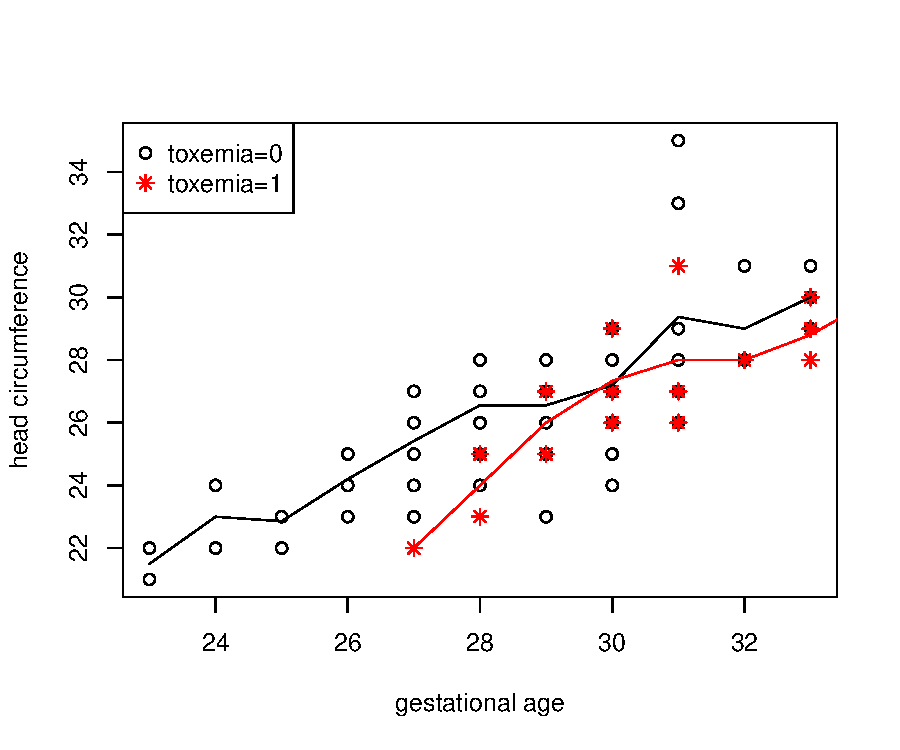
\includegraphics[width=\maxwidth]{figure/unnamed-chunk-11-1} 

}




{\centering 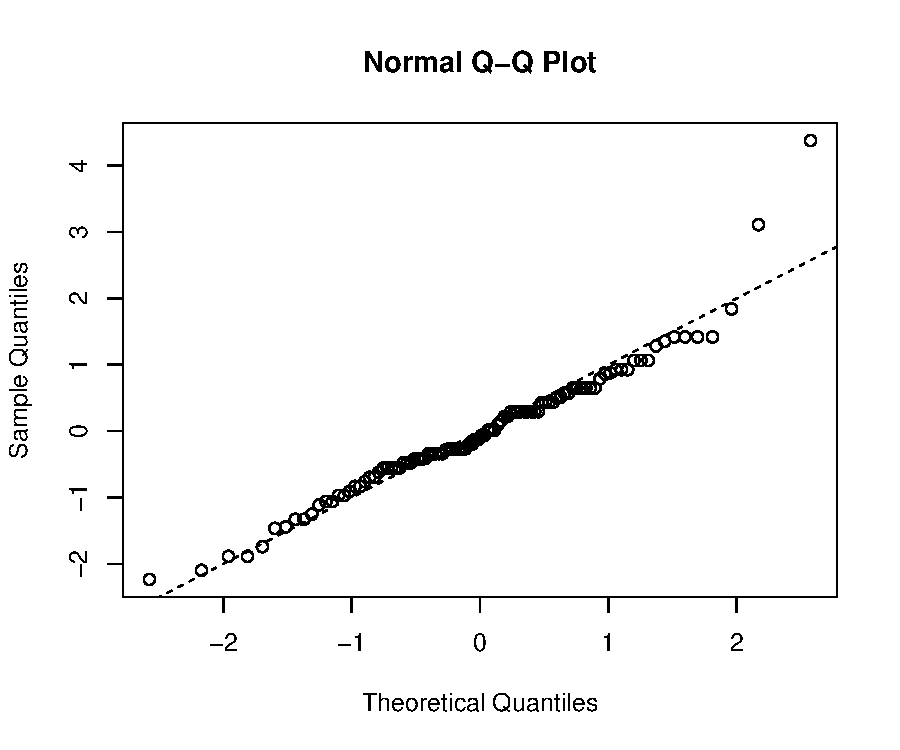
\includegraphics[width=\maxwidth]{figure/unnamed-chunk-11-2} 

}


\end{knitrout}
% \end{noindent}

\subsection*{\circled{4} Inference}
\begin{itemize}
    \item Under suitable assumptions, the fitted regression parameters are asymptotically
          normally distributed:
          \begin{align*}
              \hat{\Vector{\beta}} & \sim \MVN{\Vector{\beta},\sigma^2(\Matrix{X}^\top \Matrix{X})^{-1}},                                              \\
              \hat{\beta}_j        & \sim \N{\beta_j,\sigma^2v_{jj}},\qquad\text{where $v_{jj}=\bigl[(\Matrix{X}^\top\Matrix{X})^{-1}\bigr]_{(j,j)}$}.
          \end{align*}
    \item Since $ \sigma^2 $ is generally unknown, we replace it with the unbiased estimate $ \hat{\sigma}^2 $, and obtain $ \se{\hat{\beta}_j}=\sqrt{\hat{\sigma}^2v_{jj}} $.
    \item The inference is then based on the $t$-distribution result:
          \[ \frac{\hat{\beta}_j-\beta_j}{\se{\hat{\beta}_j}}\sim t_{n-p-1}.  \]
\end{itemize}
\subsubsection*{Low Birthweight Infant Data Example}
\begin{itemize}
    \item Is there a significant (linear) relationship between head circumference and
          gestational age?

          We wish to test $ \HN $: $ \beta_1=0 $ vs $ \HA $: $ \beta_1\ne 0 $.
          \[ t=\frac{\hat{\beta}_1-(0)}{\se{\hat{\beta}_1}}\sim t_{98}, \]
          if $ \HN $ is true, and we reject $ \HN $ if $ \abs{t}>t_{98,0.975}=1.985 $.
          Here we have $ t=0.78/0.063=12.37\gg 1.985 $, so we reject $ \HN $.
    \item What is the \qty{95}{\percent} confidence interval for the expected increase in head
          circumference when the gestational age of a baby increases by 1 week?

          A \qty{95}{\percent} CI for $ \beta_1 $:
          \[ \hat{\beta}_1\pm t_{98,0.975}\se{\hat{\beta}_1}=0.78\pm 1.985(0.063)=(0.665,0.905). \]
\end{itemize}

\subsection*{Linear models with multiple predictors}
\subsubsection*{Low Birthweight Infant Data Example}
\begin{itemize}
    \item \emph{Toxemia}, a pregnancy complication characterized by high blood pressure
          and signs of damage to liver and kidneys, may also have an impact on the
          development of babies.
          %\begin{noindent}
\begin{knitrout}
\definecolor{shadecolor}{rgb}{0.969, 0.969, 0.969}\color{fgcolor}

{\centering 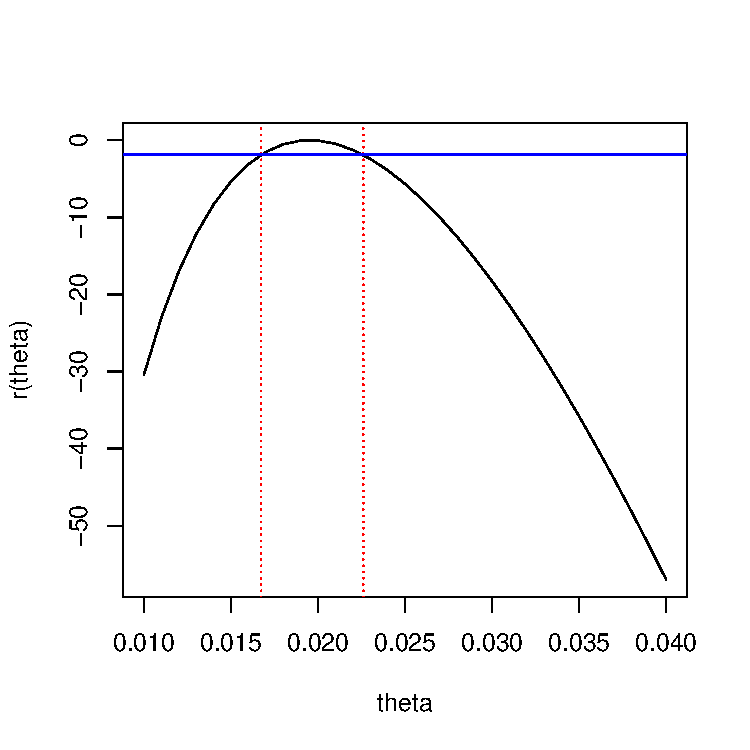
\includegraphics[width=\maxwidth]{figure/unnamed-chunk-12-1} 

}


\end{knitrout}
          %\end{noindent}
    \item Does \emph{toxemia}, after adjustment for gestational age, also affect the head
          circumference?
\begin{knitrout}
\definecolor{shadecolor}{rgb}{0.969, 0.969, 0.969}\color{fgcolor}\begin{kframe}
\begin{alltt}
\hlstd{fit} \hlkwb{<-} \hlkwd{lm}\hlstd{(headcirc} \hlopt{~} \hlstd{gestage} \hlopt{+} \hlkwd{factor}\hlstd{(toxemia),} \hlkwc{data} \hlstd{= lowbwt)}
\hlkwd{summary}\hlstd{(fit)}
\end{alltt}
\begin{verbatim}

Call:
lm(formula = headcirc ~ gestage + factor(toxemia), data = lowbwt)

Residuals:
    Min      1Q  Median      3Q     Max 
-3.8427 -0.8427 -0.0525  0.8109  6.4092 

Coefficients:
                 Estimate Std. Error t value Pr(>|t|)    
(Intercept)       1.49558    1.86799   0.801  0.42530    
gestage           0.87404    0.06561  13.322  < 2e-16 ***
factor(toxemia)1 -1.41233    0.40615  -3.477  0.00076 ***
---
Signif. codes:  0 '***' 0.001 '**' 0.01 '*' 0.05 '.' 0.1 ' ' 1

Residual standard error: 1.507 on 97 degrees of freedom
Multiple R-squared:  0.6528,	Adjusted R-squared:  0.6456 
F-statistic: 91.18 on 2 and 97 DF,  p-value: < 2.2e-16
\end{verbatim}
\end{kframe}
\end{knitrout}
          What is the interpretation of $ \beta_2 $?

          $ \hat{\beta}_3=-1.41233 $. After adjustment of gestational age, the babies whose mothers had toxemia have smaller (by \qty{1.41}{\cm}) than
          those whose mothers did not. This difference is significant (test $ \HN $: $ \beta_2=0 $, $ p\text{-value}=0.0076<0.05$).
    \item Is the rate of increase of head circumference with gestational age the same
          for infants whose mothers with toxemia as those whose mother without it?
          \[ Y_i=\beta_0+\beta_1x_{i1}+\beta_2x_{i2}+\beta_3x_{i1}x_{i2}+\varepsilon_i. \]
\begin{knitrout}
\definecolor{shadecolor}{rgb}{0.969, 0.969, 0.969}\color{fgcolor}\begin{kframe}
\begin{alltt}
\hlstd{fit} \hlkwb{<-} \hlkwd{lm}\hlstd{(headcirc} \hlopt{~} \hlstd{gestage} \hlopt{*} \hlkwd{factor}\hlstd{(toxemia),} \hlkwc{data} \hlstd{= lowbwt)}
\hlkwd{summary}\hlstd{(fit)}
\end{alltt}
\begin{verbatim}

Call:
lm(formula = headcirc ~ gestage * factor(toxemia), data = lowbwt)

Residuals:
    Min      1Q  Median      3Q     Max 
-3.8366 -0.8366 -0.0928  0.7910  6.4341 

Coefficients:
                         Estimate Std. Error t value Pr(>|t|)    
(Intercept)               1.76291    2.10225   0.839    0.404    
gestage                   0.86461    0.07390  11.700   <2e-16 ***
factor(toxemia)1         -2.81503    4.98515  -0.565    0.574    
gestage:factor(toxemia)1  0.04617    0.16352   0.282    0.778    
---
Signif. codes:  0 '***' 0.001 '**' 0.01 '*' 0.05 '.' 0.1 ' ' 1

Residual standard error: 1.515 on 96 degrees of freedom
Multiple R-squared:  0.6531,	Adjusted R-squared:  0.6422 
F-statistic: 60.23 on 3 and 96 DF,  p-value: < 2.2e-16
\end{verbatim}
\end{kframe}
\end{knitrout}
          What is the interpretation of $ \beta_3 $?

          $ \beta_3 $ is the differences in slopes between the two groups (\lstinline{toxemia=1} vs \lstinline{toxemia=0}).
          We want to test $ \HN $: $ \beta_3=0 $, $ t=0.282 $, $ p\text{-value}=0.778>0.05 $. No evidence to reject $ \HN $.
\end{itemize}

\subsection*{Limitations of Linear Regression}
Linear regression models can be very useful but may not be appropriate to use
when response $ Y $ is not continuous and can not be assumed to be normally
distributed, e.g.,
\begin{itemize}
    \item Binary data ($ Y=0 $ or $ Y=1 $),
    \item Count data ($ Y=0,1,2,3,\ldots $).
\end{itemize}
\textcolor{Red}{Generalized Linear Models (GLM)} extend the linear regression framework to
address the above issue.
\begin{itemize}
    \item Suitable for continuous and discrete data.
    \item Normal/Gaussian linear regression is a special case of GLM.
    \item Inference based on maximum likelihood methods (review next class --- 431
          Appendix, Stat 330 notes).
\end{itemize}

\makeheading{Week 2}{\daterange{2021-09-13}{2021-09-17}}
\section*{Topic 1b: Review of Likelihood Methods}
\addcontentsline{toc}{section}{Topic 1b: Review of Likelihood Methods}
\subsection*{Distributions with a Single Parameter}
\begin{Regular}{Setup}
      \begin{itemize}
            \item Suppose $ Y $ is a random variable with probability density (or mass) function
                  $ f(y;\theta) $, where $ \theta\in\Omega $ is a continuous parameter.
            \item The true value of $ \theta $ is unknown.
            \item We wish to make inferences about $ \theta $ (i.e., we may want to estimate $ \theta $, calculate
                  a \qty{95}{\percent} CI or carry out tests of hypotheses regarding $ \theta $).
      \end{itemize}
\end{Regular}
\subsection*{Likelihood Function}
\begin{itemize}
      \item The \textcolor{Red}{Likelihood function} is any function which is proportional to the probability
            of observing the data one actually obtained, i.e.,
            \[ L(\theta;y)=cf(y;\theta)=c\Prob{Y=y;\theta}, \]
            where $ c $ is a \emph{proportionality constant} that does not depend on $ \theta $.
      \item $ L(\theta;y) $ contains all the information regarding $ \theta $ from the data.
      \item $ L(\theta;y) $ ranks the various parameter values in terms of their consistency
            with the data.
      \item Since $ L(\theta;y) $ is defined in terms of the random variable $ y $, it is itself a
            random variable.
\end{itemize}
\subsection*{Maximum Likelihood Estimator}
\begin{itemize}
      \item For the purposes of estimation we typically want to find $ \theta $ value that makes the
            observed data the most likely (hence the term \textcolor{Red}{maximum likelihood}).
      \item The \textcolor{Red}{maximum likelihood estimator (MLE)} of $ \theta $ is
            \[ \hat{\theta}=\argmax_\theta L(\theta;y). \]
      \item Estimation becomes a simple optimization problem!
      \item It is often easier to work with the logarithm of the likelihood function, i.e., the
            \textcolor{Red}{log-likelihood function}
            \[ \ell(\theta;y)=\log[\big]{L(\theta;y)}. \]
      \item Equivalently, since the $ \log{\:\cdot\:} $ function is monotonic, the value of $ \theta $ that maximizes $ L(\theta;y) $ also
            maximizes the log-likelihood $ \ell(\theta;y) $.
      \item For simplicity, we drop the $ y $ and use $ L(\theta)=L(\theta;y) $ and $ \ell(\theta)=\ell(\theta;y) $.
\end{itemize}

\subsection*{A List of Important Functions}
\begin{itemize}
      \item \textcolor{Red}{Log-likelihood function}: $ \ell(\theta)=\log[\big]{L(\theta)} $.
      \item \textcolor{Red}{Score function}: $ S(\theta)=\pdv{\ell(\theta)}{\theta}=\ell^\prime(\theta)$.
      \item \textcolor{Red}{Information function}: $ I(\theta)=-\pdv[order=2]{\ell(\theta)}{\theta}=-\ell^{\prime\prime}(\theta) $.
      \item \textcolor{Red}{Fisher information function}: $ \mathcal{I}(\theta)=\E[\big]{I(\theta)} $.
      \item \textcolor{Red}{Relative likelihood function}: $ R(\theta)=L(\theta)/L(\hat{\theta}) $.
      \item \textcolor{Red}{Log relative likelihood function}: $ r(\theta)=\log[\big]{L(\theta)/L(\hat{\theta})}=\ell(\theta)-\ell(\hat{\theta}) $.
\end{itemize}
\subsection*{Maximum Likelihood Estimation}
\begin{itemize}
      \item Want $ \theta $ that maximizes $ \ell(\theta) $, or equivalently solves $ S(\theta)=0 $.
      \item Sometimes $ S(\theta)=0 $ can be solved explicitly (easy in this case), but often we must solve iteratively.
      \item Check that the solution corresponds to a maxima of $ \ell(\theta) $ by verifying the value of the second derivative at $ \hat{\theta} $ is negative, or
            \[ I(\hat{\theta})=-\ell^{\prime\prime}(\hat{\theta})>0. \]
      \item \textcolor{Red}{Invariance property of MLEs}: if $ g(\theta) $ is any function of the parameter $ \theta $, then the MLE of $ g(\theta) $ is $ g(\hat{\theta}) $.
            \begin{Example}{}
                  If $ \hat{\theta} $ is the MLE of $ \theta $, then $ e^{\hat{\theta}} $ is the MLE of $ e^{\theta} $.
            \end{Example}
\end{itemize}
\subsection*{Example: Binomial Distribution}
\begin{Example}{Example: Binomial Distribution}
      \begin{itemize}
            \item A study was conducted to examine the risk for hormone use in healthy
                  postmenopausal women.
            \item Suppose a group of $ n $ women received a combined hormone therapy, and were
                  monitored for the development of breast cancer during 8.5 years followup.
            \item Let
                  \[ Y_i=\begin{cases*}
                              1 & , if woman $ i $ developed breast cancer, \\
                              0 & , otherwise,
                        \end{cases*} \]
                  for $ i=1,\ldots,n $.
            \item Suppose $ Y_i \iid\Bernoulli{\pi} $ where $ \pi=\Prob{Y_i=1} $, then the total number of woman developed breast cancer is:
                  \[ Y=\sum_{i=1}^{n} Y_i \sim \Binomial{n,\pi}. \]
            \item We wish to find the MLE of unknown parameter $ \pi $ (probability of cancer).
      \end{itemize}
\end{Example}
\begin{itemize}
      \item \textcolor{Red}{Likelihood function}:
            \[ L(\pi;y)=c\Prob{Y=y;\pi}=\pi^y(1-\pi)^{n-y}, \]
            where we take $ c=1/\binom{n}{y} $ to simplify the likelihood.
      \item \textcolor{Red}{Log-likelihood function}:
            \[ \ell(\pi)=y\log{\pi}+(n-y)\log{1-\pi}. \]
      \item \textcolor{Red}{Score function}:
            \[ S(\pi)=\frac{y}{\pi}-\frac{n-y}{1-\pi}.  \]
      \item \textcolor{Red}{Maximum Likelihood Estimator}:
            \[ S(\pi)=0\implies \hat{\pi}=\frac{\sum_{i=1}^{n} y_i}{n}=\bar{y}. \]
      \item Second derivative test using \textcolor{Red}{information function}:
            \[ I(\pi)=-\ell^{\prime\prime}(\pi)=\frac{y}{\pi^2}+\frac{n-y}{(1-\pi)^2}>0\ \forall \pi\in(0,1). \]
\end{itemize}
\begin{Example}{Example: Hormone Therapy Data}
      \begin{itemize}
            \item A group of $ n=8506 $ postmenopausal women aged 50-79 received EPT and $ Y=166 $
                  developed invasive breast cancer during the followup.
            \item Assume $ Y \sim \Binomial{n,\pi} $ with unknown parameter $ \pi $.
            \item The \textcolor{Red}{maximum likelihood estimate} of $ \pi $ is:
                  \[ \hat{\pi}=\bar{y}=\frac{y}{n} =\frac{166}{8506}=0.0195. \]
      \end{itemize}
\end{Example}
\subsection*{Example: Poisson Distribution}
Suppose $ y_1,\ldots,y_n $ is an iid sample from a Poisson distribution with probability mass function:
\[ f(y;\lambda)=\Prob{Y=y;\lambda}=\frac{\lambda^y e^{-\lambda}}{y!},\; \lambda>0,\,y=0,1,2,\ldots.  \]
\begin{itemize}
      \item \textcolor{Red}{Likelihood function}:
            \[ L(\lambda;y_1,\ldots,y_n)=\prod_{i=1}^n f(y_i;\lambda)=\frac{\lambda^{\sum y_i}e^{-n\lambda}}{\prod_i y_i!}.  \]
      \item \textcolor{Red}{Log-likelihood function}:
            \[ \ell(\lambda)=\biggl(\sum_i y_i\biggr)\log{\lambda}-n\lambda-\sum_{i=1}^{n} \log{y_i!}. \]
      \item \textcolor{Red}{Score function}:
            \[ S(\lambda)=\frac{\sum_i y_i}{\lambda}-n=0\implies \hat{\lambda}=\frac{\sum_{i=1}^{n} y_i}{n} =\bar{y}.  \]
\end{itemize}
\subsection*{Newton Raphson Algorithm For Finding MLE}
\begin{itemize}
      \item Sometimes, solving $ S(\theta)=0 $ can be challenging and closed form solutions may
            not be obtained, iterative method need to be used to find the MLE.
      \item Recall \textcolor{Red}{Taylor Series} expansion of a differentiable function $ f(x) $ about a point $ a $:
            \[ f(x)=f(a)+\frac{f^\prime(a)}{1!}(x-a)+\frac{f^{\prime\prime}(a)}{2!}(x-a)^2+\cdots.  \]
      \item Now suppose we wish to find $ \hat{\theta} $, the root of $ S(\theta)=0 $ and $ \theta^{(0)} $ is a guess that
            is ``close'' to $ \hat{\theta} $.
      \item Consider the Taylor series expansion of $ S(\theta) $ about $ \theta^{(0)} $:
            \[ S(\theta)=S(\theta^{(0)})+\frac{S^{\prime}(\theta^{(0)})}{1!}(\theta-\theta^{(0)})+\frac{S^{\prime\prime}(\theta^{(0)})}{2!}(\theta-\theta^{(0)})^2+\cdots.   \]
      \item For $ \abs{\theta-\theta^{(0)}} $ very small, the second and higher order terms can be dropped to a good approximation:
            \begin{align*}
                  S(\theta) & \simeq S(\theta^{(0)})+S^\prime(\theta^{(0)})(\theta-\theta^{(0)}). \\
                  S(\theta) & \simeq S(\theta^{(0)})-I(\theta^{(0)})(\theta-\theta^{(0)}).
            \end{align*}
      \item Then at $ \theta=\hat{\theta} $,
            \begin{align*}
                  S(\hat{\theta})                            & \simeq S(\theta^{(0)})-I(\theta^{(0)})(\hat{\theta}-\theta^{(0)}) \\
                  I(\theta^{(0)})(\hat{\theta}-\theta^{(0)}) & \simeq S(\theta^{(0)})                                            \\
                  (\hat{\theta}-\theta^{(0)})                & \simeq I^{-1}(\theta^{(0)})S(\theta^{(0)})                        \\
                  \hat{\theta}                               & \simeq \theta^{(0)}+I^{-1}(\theta^{(0)})S(\theta^{(0)}).
            \end{align*}
      \item This suggests a revised guess for $ \hat{\theta} $ is:
            \[ \theta^{(1)}=\theta^{(0)}+I^{-1}(\theta^{(0)})S(\theta^{(0)}) \]
\end{itemize}
\begin{Regular}{Newton Raphson Algorithm for finding the MLE}
      \begin{itemize}
            \item Begin with an initial estimate $ \theta^{(0)} $.
            \item Iteratively obtain updated estimate by using:
                  \[ \theta^{(i+1)}=\theta^{(i)}+I^{-1}(\theta^{(i)})S(\theta^{(i)}). \]
            \item Iteration continues until $ \theta^{(i+1)}\simeq \theta^{(i)} $ within a specified tolerance.
            \item Then set $ \hat{\theta}=\theta^{(i+1)} $, check that $ I(\hat{\theta})>0 $.
      \end{itemize}
\end{Regular}
\subsection*{Inference for Scalar Parameters $ \theta $}
\begin{itemize}
      \item So far we have discussed estimation of $ \hat{\theta} $, next we want to conduct inference
            about $ \theta $, i.e., carry out hypothesis tests and construct confidence intervals of $ \theta $.
      \item Likelihood inference relies on the following \textcolor{Red}{asymptotic distribution results}:
            \begin{Regular}{Useful asymptotic distributional results}
                  \begin{itemize}
                        \item \textcolor{Red}{(log) Likelihood ratio statistic}: $ -2\log[\big]{R(\theta)}=-2r(\theta)\sim \chi^2_{(1)} $.
                        \item \textcolor{Red}{Score statistic}: $ \bigl(S(\theta)\bigr)^2/I(\theta)\sim \chi^2_{(1)} $.
                        \item \textcolor{Red}{Wald statistic}: $ (\hat{\theta}-\theta)^2 I(\hat{\theta}) \sim \chi^2_{(1)} $ or $ (\hat{\theta}-\theta)\sqrt{I(\hat{\theta})}\sim \N{0,1} $
                              since $ Z \sim \N{0,1} \implies Z^2 \sim \chi^2_{1} $.
                  \end{itemize}
            \end{Regular}
\end{itemize}
\subsection*{Confidence Interval (CI)}
Suppose we want a $ 100(1-\alpha)\, \% $ confidence interval for $ \theta $.
\begin{itemize}
      \item The \textcolor{Red}{Likelihood ratio (LR)} based pivotal gives a confidence interval:
            \[ \Set*{\theta:-2r(\theta)<\chi^2_{1}(1-\alpha)}, \]
            where $ \chi^2_1(1-\alpha) $ is the upper $ \alpha $ percentage point of the $ \chi^2_1 $ distribution.
      \item The \textcolor{Red}{Wald}-based pivotal gives an interval:
            \[ \Set*{\theta:(\hat{\theta}-\theta)^2 I(\hat{\theta})<\chi^2_1(1-\alpha)}, \]
            or equivalently
            \[ \hat{\theta}\pm Z_{1-\alpha/2}\bigl(I(\hat{\theta})\bigr)^{-1/2}, \]
            where $ Z_{1-\alpha/2} $ is the upper $ \alpha/2 $ percentage point of the standard normal.
\end{itemize}
\subsection*{Example: Hormone Therapy Data}
\textcolor{Red}{Likelihood Ratio} based $ \qty{95}{\percent} $ CI: $ \Set*{\theta:-2r(\theta)<\chi^2_{1}(0.95)} $
where $ r(\theta)=\ell(\theta)-\ell(\hat{\theta}) $.
\begin{itemize}
      \item For the Binomial distribution: $ \hat{\theta}=y/n $, and
            \[ r(\theta)=\bigl(y\log{\theta}+(n-y)\log{1-\theta}\bigr)-\biggl(y\log*{\frac{y}{n}}+(n-y)\log*{1-\frac{y}{n}}\biggr). \]
      \item To find the root of $ -2r(\theta)=\chi^2_1(0.95) $:
            %\begin{noindent}
\begin{knitrout}
\definecolor{shadecolor}{rgb}{0.969, 0.969, 0.969}\color{fgcolor}\begin{kframe}
\begin{alltt}
\hlstd{y} \hlkwb{=} \hlnum{166}
\hlstd{n} \hlkwb{=} \hlnum{8506}
\hlstd{LRCI} \hlkwb{=} \hlkwa{function}\hlstd{(}\hlkwc{theta}\hlstd{,} \hlkwc{y}\hlstd{,} \hlkwc{n}\hlstd{) \{}
  \hlopt{-}\hlnum{2} \hlopt{*} \hlstd{(y} \hlopt{*} \hlkwd{log}\hlstd{(theta)} \hlopt{+} \hlstd{(n} \hlopt{-} \hlstd{y)} \hlopt{*} \hlkwd{log}\hlstd{(}\hlnum{1} \hlopt{-} \hlstd{theta)} \hlopt{-} \hlstd{y} \hlopt{*} \hlkwd{log}\hlstd{(y}\hlopt{/}\hlstd{n)} \hlopt{-}
    \hlstd{(n} \hlopt{-} \hlstd{y)} \hlopt{*} \hlkwd{log}\hlstd{(}\hlnum{1} \hlopt{-} \hlstd{y}\hlopt{/}\hlstd{n))} \hlopt{-} \hlkwd{qchisq}\hlstd{(}\hlnum{0.95}\hlstd{,} \hlnum{1}\hlstd{)}
\hlstd{\}}
\hlstd{mle} \hlkwb{=} \hlstd{y}\hlopt{/}\hlstd{n}
\hlkwd{uniroot}\hlstd{(LRCI,} \hlkwd{c}\hlstd{(}\hlnum{0}\hlstd{, mle),} \hlkwc{y} \hlstd{= y,} \hlkwc{n} \hlstd{= n)}\hlopt{$}\hlstd{root}
\end{alltt}
\begin{verbatim}
[1] 0.01673867
\end{verbatim}
\begin{alltt}
\hlkwd{uniroot}\hlstd{(LRCI,} \hlkwd{c}\hlstd{(mle,} \hlnum{1}\hlstd{),} \hlkwc{y} \hlstd{= y,} \hlkwc{n} \hlstd{= n)}\hlopt{$}\hlstd{root}
\end{alltt}
\begin{verbatim}
[1] 0.02260709
\end{verbatim}
\end{kframe}
\end{knitrout}
            %\end{noindent}
      \item The likelihood ratio based $ \qty{95}{\percent} $ CI is $(0.017, 0.023)$.
\end{itemize}
\textcolor{Red}{Wald} based $ \qty{95}{\percent} $ CI: $ \hat{\theta}\pm Z_{0.975}\bigl(I(\hat{\theta})\bigr)^{-1/2} $.
\begin{itemize}
      \item For Binomial distribution $ \hat{\theta}=y/n $ and
            \[ I(\hat{\theta})=\frac{y}{\hat{\theta}^2}+\frac{n-y}{(1-\hat{\theta})^2}=n^2\biggl(\frac{1}{y} +\frac{1}{n-y}\biggr).   \]
      \item So we solve:
            \begin{align*}
                  \hat{\theta}\pm 1.96\bigl(I(\hat{\theta})\bigr)^{-1/2}
                   & =0.0195 \pm 1.96(0.0015) \\
                   & =(0.017, 0.022).
            \end{align*}
      \item The Wald based $ \qty{95}{\percent} $ CI is: $ (0.017, 0.022) $.
            \begin{figure}[!htbp]
                  \centering
                  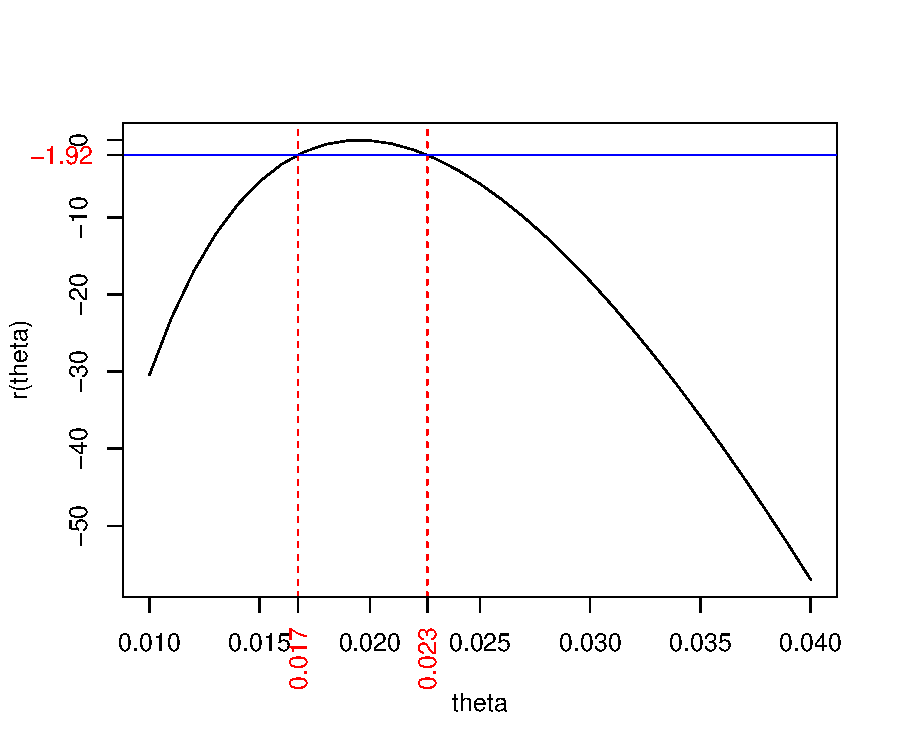
\includegraphics{figures/1bLR.pdf}
            \end{figure}
\end{itemize}
\subsection*{Hypotheses Test}
Suppose we are interested in testing hypotheses:
\[ \text{$\HN$: $\theta=\theta_0$ vs $\HA$: $\theta\ne \theta_0$.} \]
\begin{itemize}
      \item \textcolor{Red}{Likelihood ratio (LR) test}: $ p\text{-value}=\Prob*{\chi^2_1>-2r(\theta_0)} $.
      \item \textcolor{Red}{Score test}: $ p\text{-value}=\Prob*{\chi^2_1>\bigl(S(\theta)\bigr)^2/I(\theta_0)} $.
      \item \textcolor{Red}{Wald test}:
            \[ p\text{-value}=\Prob*{\chi^2_1>(\hat{\theta}-\theta_0)^2 I(\hat{\theta})}\text{, or }
                  p\text{-value}=\Prob*{\abs{Z}>\abs{\hat{\theta}-\theta_0}\sqrt{I(\hat{\theta})}}. \]
\end{itemize}
\subsection*{Example: Hormone Therapy Data}
Suppose we wish to test if women received EPT would have a risk of breast
cancer same as that of the general population, say about \qty{1.5}{\percent}.
\[ \text{$\HN$: $\theta=0.015$ vs $\HA$: $\theta\ne 0.015$.} \]
\begin{itemize}
      \item \textcolor{Red}{Likelihood Ratio} based test:
            \begin{align*}
                  r(\theta_0=0.015)
                   & =\biggl(y\log{0.015}+(n-y)\log{1-0.15}\biggr)-\biggl(y\log*{\frac{y}{n}}+(n-y)\log*{1-\frac{y}{n} }\biggr) \\
                   & =-5.3637.
            \end{align*}
            Thus, the $ p $-value for the test is given by:
            \[ p=\Prob*{\chi^2_{(1)}>-2r(0.015)}=\Prob*{\chi^2_{(1)}>10.7274}=0.001. \]
            Therefore, we \emph{reject} $ \HN $ and conclude that the risk of breast cancer for women received EPT is
            significantly different from \qty{1.5}{\percent}.
\end{itemize}
\subsection*{Notes on Asymptotic Inference}
\begin{itemize}
      \item Asymptotic results: approximation improves as sample size increases.
      \item Results are exact for a Normal linear model if $ \theta $ is the mean parameter and $ \sigma^2 $ is
            known.
      \item \textcolor{Red}{LR approach}:
            \begin{itemize}
                  \item Need to evaluate (log) likelihood at two locations.
                  \item Not always a closed from solution for a CI.
                  \item Usually the best approach.
            \end{itemize}
      \item \textcolor{Red}{Score approach}:
            \begin{itemize}
                  \item Usually the least powerful test.
                  \item Don't actually need to find MLE to use.
            \end{itemize}
      \item \textcolor{Red}{Wald's approach}:
            \begin{itemize}
                  \item Always get a closed form solution for a CI.
                  \item May not behave well for skewed likelihoods (transform?).
            \end{itemize}
      \item All three are asymptotically equivalent!
\end{itemize}
\subsection*{Likelihood Methods for Parameter Vectors}
Suppose $ \Vector{\theta}\in \Omega $ is a continuous $ p\times 1 $ parameter vector
indexing a probability density (or mass) function $ f(\Vector{y};\Vector{\theta}) $. The likelihood and
log-likelihood functions are defined as before, but
\begin{itemize}
      \item $ \Vector{S}(\Vector{\theta})=\pdv{\ell( \Vector{\theta})}{ \Vector{\theta}} $ is the $ p\times 1 $ \textcolor{Red}{Score vector}, i.e.,
            \[ \Vector{S}(\Vector{\theta})=\begin{bmatrix}
                        \pdv{\ell(\theta)}{\theta_1} \\
                        \vdots                       \\
                        \pdv{\ell(\theta)}{\theta_p}
                  \end{bmatrix}. \]
      \item $ \Matrix{I}(\Vector{\theta})=-\pdv{\ell(\Vector{\theta})}{ \Vector{\theta}^\top,\Vector{\theta}} $ is the $ p\times p $ \textcolor{Red}{Information matrix}, i.e.,
            \[ \Matrix{I}(\Vector{\theta})=\begin{bmatrix}
                        -\pdv[order=2]{\ell(\theta)}{\theta_1} & -\pdv{\ell(\theta)}{\theta_1,\theta_2} & \cdots & \pdv{\ell(\theta)}{\theta_1,\theta_p} \\
                                                               & -\pdv[order=2]{\ell(\theta)}{\theta_2} & \cdots & \pdv{\ell(\theta)}{\theta_1,\theta_p} \\
                                                               &                                        & \ddots & \pdv[order=2]{\ell(\theta)}{\theta_p}
                  \end{bmatrix}. \]

\end{itemize}
\begin{itemize}
      \item The Newton Raphson algorithm applies as before, but with vectors and matrices
            as follows:
            \[ \Vector{\theta}^{(i+1)}=\Vector{\theta}^{(i)}+\Matrix{I}^{-1}(\Vector{\theta}^{(i)})\Vector{S}(\Vector{\theta}^{(i)}). \]
      \item Again, we apply iteratively until we obtain convergence, but now check to
            see if $ \Matrix{I}(\hat{\Vector{\theta}}) $ is a positive definite matrix.
      \item Analogs to the LR, Score and Wald results apply based on partitioning the
            Information matrix by $ \Vector{\theta}=(\Vector{\alpha},\Vector{\beta})^\top $,
            where $ \Vector{\alpha} $ is a $ p\times 1 $ vector of nuisance parameters and $ \Vector{\beta} $ is a $ q\times 1 $ vector of parameters of interest:
            \[ \Matrix{I}=\Matrix{I}(\Vector{\alpha},\Vector{\beta})=\begin{pmatrix}
                        \Matrix{I}_{\Vector{\alpha}\Vector{\alpha}}(\Vector{\alpha},\Vector{\beta}) & \Matrix{I}_{\Vector{\alpha}\Vector{\beta}}(\Vector{\alpha},\Vector{\beta}) \\
                        \Matrix{I}_{\Vector{\beta}\Vector{\alpha}}(\Vector{\alpha},\Vector{\beta})  & \Matrix{I}_{\Vector{\beta}\Vector{\beta}}(\Vector{\alpha},\Vector{\beta})
                  \end{pmatrix}, \]
            where
            $ \Matrix{I}_{\Vector{\alpha}\Vector{\alpha}}(\Vector{\alpha},\Vector{\beta})=-\pdv{\ell}{\Vector{\alpha},\Vector{\alpha}^\top} $ is $ p\times p $,
            $ \Matrix{I}_{\Vector{\alpha}\Vector{\beta}}(\Vector{\alpha},\Vector{\beta})=-\pdv{\ell}{\Vector{\alpha},\Vector{\beta}^\top} $ is $ p\times q $,
            $ \Matrix{I}_{\Vector{\beta}\Vector{\alpha}}(\Vector{\alpha},\Vector{\beta})=-\pdv{\ell}{\Vector{\beta},\Vector{\alpha}^\top} $ is $ q\times p $, and
            $ \Matrix{I}_{\Vector{\beta}\Vector{\beta}}(\Vector{\alpha},\Vector{\beta})=-\pdv{\ell}{\Vector{\beta},\Vector{\beta}^\top} $ is $ q\times q $.
\end{itemize}

\section*{Topic 2a: Formulation of Generalized Linear Models}
\addcontentsline{toc}{section}{Topic 2a: Formulation of Generalized Linear Models}
\subsection*{The Exponential Family}
\begin{Regular}{Definition (Exponential Family)}
    Consider a random variable $ Y $ with probability density (or mass) function $ f(y;\theta,\phi) $,
    we say that the distribution is a member of the \textcolor{Red}{exponential family} if we can write
    \[ f(y;\theta,\phi)=\exp*{\frac{y\theta-b(\theta)}{a(\phi)}+c(y;\phi)}, \]
    for some functions $ a(\:\cdot\:) $, $ b(\:\cdot\:) $, and $ c(\:\cdot\:) $.
    \begin{itemize}
        \item The parameter $ \theta $ is called the \textcolor{Red}{canonical} parameter, and it is unknown.
        \item The parameter $ \phi $ is called the \textcolor{Red}{scale/dispersion} parameter, is constant, and assumed to be known.
    \end{itemize}
\end{Regular}
Many well known distributions (continuous/discrete) can be shown to be a
member of the exponential family.
\subsection*{Examples}
\begin{itemize}
    \item Poisson Distribution: $ Y \sim \Poisson{\lambda} $,
          \[ f(y;\lambda)=\frac{\lambda^y e^{-\lambda}}{y!},\; \lambda>0,\, y=0,1,\ldots.  \]
          Show that Poisson is a member of exponential family and identify the canonical
          parameter and the functions $ a(\:\cdot\:) $, $ b(\:\cdot\:) $, and $ c(\:\cdot\:) $.

          \textbf{Solution.} $ f(y;\lambda)=\exp[\big]{\log{f(y;\lambda)}}=\exp*{\frac{y\log{\lambda}-\lambda}{1} -\log{y!}} $. Therefore,
          \begin{align*}
              \theta    & =\log{\lambda}\qquad\text{(canonical/natural parameter)}, \\
              b(\theta) & =\lambda=e^{\theta},                                      \\
              \phi      & =1,                                                       \\
              a(\phi)   & =1,                                                       \\
              c(y;\phi) & =-\log{y!}.
          \end{align*}
    \item Normal Distribution: $ Y \sim \N{\mu,\sigma^2} $ and $ \sigma^2 $ known,
          \[ f(y;\theta,\phi)=\frac{1}{\sqrt{2\pi\sigma^2}}\exp*{-\frac{(y-\mu)^2}{2\sigma^2}}. \]
          Show that this Normal distribution is a member of the exponential family.

          \textbf{Solution.}
          \begin{align*}
              f(y;\mu,\sigma^2)
               & =\exp*{-\frac{y^2-2\mu y+\mu^2}{\sigma^2}-\frac{1}{2} \log{2\pi\sigma^2}}                   \\
               & =\exp*{\frac{y\mu-\mu^2/2}{\sigma^2}-\frac{y^2}{2\sigma^2}-\frac{1}{2} \log{2\pi\sigma^2}}.
          \end{align*}
          Therefore,
          \begin{align*}
              \theta    & =\mu,                                                   \\
              \phi      & =\sigma^2,                                              \\
              a(\phi)   & =\phi=\sigma^2,                                         \\
              b(\theta) & =\frac{\mu^2}{2}=\frac{\theta^2}{2},                    \\
              c(y;\phi) & =-\frac{y^2}{2\sigma^2}-\frac{1}{2} \log{2\pi\sigma^2}.
          \end{align*}
\end{itemize}
\subsection*{Properties of Exponential Family}
Consider a single observation $y$ from the exponential family.
\begin{align*}
    L(\theta,\phi;y)    & =f(y;\theta,\phi)=\exp*{\frac{y\theta-b(\theta)}{a(\phi)}+c(y;\phi)}.      \\
    \ell(\theta,\phi;y) & =\log[\big]{f(y;\theta,\phi)}=\frac{y\theta-b(\theta)}{a(\phi)}+c(y;\phi). \\
    S(\theta)           & =\pdv{\ell}{\theta}=\frac{y-b^\prime(\theta)}{a(\phi)}.                    \\
    I(\theta)           & =-\pdv[order=2]{\ell}{\theta}=\frac{b^{\prime\prime}(\theta)}{a(\phi)}.    \\
    \mathcal{I}(\theta) & =\E*{-\pdv[order=2]{\ell}{\theta}}=I(\theta).
\end{align*}
\subsection*{Some General Results for Score and Information}
\begin{Result}{Result \# 1}
    The expectation of the score function is zero.
    \[ \E[\big]{S(\theta)}=0. \]
    \tcblower{}
    \textbf{Proof}:
    \begin{align*}
        \int f(y;\theta,\phi)\odif{y}                                                         & =1                               \\
        \pdv*{\int f(y;\theta,\phi)\odif{y}}{\theta}                                          & =0                               \\
        \int\pdv*{f(y;\theta,\phi)}{\theta} \odif{y}                                          & =0                               \\
        \int\biggl(\pdv*{\log[\big]{f(y;\theta,\phi)}}{\theta}\biggr)f(y;\theta,\phi)\odif{y} & =0 &  & \label{2a:eq1}\tag*{(1)} \\
        \int S(\theta)f(y;\theta,\phi)\odif{y}                                                & =0                               \\
        \E[\big]{S(\theta)}                                                                   & =0
    \end{align*}
\end{Result}
\begin{Result}{Result \# 2}
    The expectation of the score function squared is the expected information.
    \[  \E[\big]{S(\theta;y)^2}=\E[\big]{I(\theta;y)} \]
    \tcblower{}
    \textbf{Proof}: Differentiate~\ref{2a:eq1} again,
    \begin{align*}
        \int\biggl(\pdv*{\log[\big]{f(y;\theta,\phi)}}{\theta}\biggr)f(y;\theta,\phi)\odif{y}                                                                                                                & =0 \\
        \int \biggl(\pdv*[order=2]{\log[\big]{f(y;\theta,\phi)}}{\theta}\biggr)f(y;\theta,\phi)\odif{y}+\int\biggl(\pdv*{\log[\big]{f(y;\theta,\phi)}}{\theta}\biggr)\pdv*{f(y;\theta,\phi)}{\theta}\odif{y} & =0 \\
        \int \pdv*[order=2]{\log[\big]{f(y;\theta,\phi)}}{\theta}f(y;\theta,\phi)\odif{y}+\int\biggl(\pdv*{f(y;\theta,\phi)}{\theta}\biggr)^2 f(y;\theta,\phi)\odif{y}                                       & =0 \\
        \int -I(\theta)f(y;\theta,\phi)\odif{y}+\int S(\theta)^2 f(y;\theta,\phi)\odif{y}                                                                                                                    & =0 \\
        \E[\big]{-I(\theta;y)}+\E[\big]{S(\theta;y)^2}                                                                                                                                                       & =0
    \end{align*}
\end{Result}
Now for the exponential family, we apply above results and obtain:
\begin{align*}
    \E[\big]{S(\theta)}                                          & =0,                                             \\
    \E*{\frac{Y-b^{\prime}(\theta)}{a(\phi)}}                    & =0,                                             \\
    \E{Y}                                                        & =b^\prime(\theta),                              \\\\
    \E[\big]{S(\theta)^2}                                        & =\E[\big]{I(\theta)},                           \\
    \E*{\biggl(\frac{Y-b^\prime(\theta)}{a(\phi)} \biggr)^{\!2}} & =\E*{\frac{b^{\prime\prime}(\theta)}{a(\phi)}}, \\
    \frac{1}{a(\phi)^2}\E*{\bigl(Y-\E{Y}\bigr)^2}                & =\frac{b^{\prime\prime}(\theta)}{a(\phi)},      \\
    \Var{Y}                                                      & =b^{\prime\prime}(\theta)a(\phi).
\end{align*}
\begin{Regular}{Mean and Variance for the Exponential Family}
    \begin{itemize}
        \item Mean: $ \E{Y}=b^\prime(\theta)=\mu $.
        \item Variance: $ \Var{Y}=b^{\prime\prime}(\theta)a(\phi) $.
    \end{itemize}
\end{Regular}
Note that:
\begin{itemize}
    \item $ b^\prime(\theta)=\mu $ tells the relationship between \emph{canonical} parameter $ \theta $ and $ \mu $.
    \item $ b^{\prime\prime}(\theta) $ is a function of $ \theta $ and hence can be also expressed as a function of $ \mu $.
    \item Thus, we write $ b^{\prime\prime}(\theta)=\V{\mu} $ and call $ \V{\mu} $ the \textcolor{Red}{variance function}.
    \item Subsequently, we have:
          \[ \Var{Y}=b^{\prime\prime}(\theta)a(\phi)=\V{\mu}a(\phi), \]
          which is the \textcolor{Red}{mean-variance relationship} for the exponential family.
\end{itemize}
\subsection*{Link Functions}
\begin{Regular}{Definition (Link Function)}
    The \textcolor{Red}{link function} relates the linear predictor $ \eta=\Vector{x}^\top\Vector{\beta} $ to the expected value $ \mu $ of the random variable $ Y $, i.e.,
    \[ g(\mu)=\eta=\Vector{x}^\top\Vector{\beta}, \]
    where $ g(\:\cdot\:) $ is the link function.
\end{Regular}
\begin{Regular}{Definition (Canonical Link Function)}
    When $Y$ is a member of the exponential family we define the \textcolor{Red}{canonical link function} to be:
    \[ g(\mu)=\theta=\eta=\Vector{x}^\top\Vector{\beta} \]
    (i.e., the choice of $ g(\:\cdot\:) $ that sets canonical parameter = linear predictor).
\end{Regular}
\subsection*{Examples}
Recall that $ \Poisson{\lambda} $ is a member of exponential family,
\[ f(y;\lambda)=\frac{\lambda^y e^{-\lambda}}{y!}=\exp*{\frac{y\log{\lambda}-\lambda}{1}-\log{y!}}  \]
where $ \theta=\log{\lambda} $, $ \phi=1 $, $ b(\theta)=\lambda=e^{\theta} $, and $ a(\phi)=1 $. Now to find the mean, variance function, and canonical link function:
\begin{itemize}
    \item \textcolor{Blue}{Mean}: $ \E{Y}=b^\prime(\theta)=e^{\theta}=\mu\implies \theta=\log{\mu} $.
    \item \textcolor{Blue}{Variance Function}: $ \V{\mu}=b^{\prime\prime}(\theta)=e^{\theta}\implies \V{\mu}=\mu $.
    \item \textcolor{Blue}{Variance}: $ \Var{Y}=\V{\mu}a(\phi)=\mu $ (mean-variance relationship).
    \item \textcolor{Blue}{Canonical link}: set $ \theta=\eta $ using $ \theta=\log{\mu}=\eta=\Vector{x}^\top \Vector{\beta} $, i.e., $ g(\mu)=\log{\mu} $ where $ \log{\:\cdot\:} $
          is the canonical link.
\end{itemize}
Moving forward, we consider a log-linear model: $ \log{\mu_i}=\Vector{x}_i^\top \Vector{\beta} $.

\subsection*{Remarks on Link Function}
\begin{itemize}
    \item We can choose any function $ g(\:\cdot\:) $ as the link function in theory.
    \item The canonical link is a special link function, we often choose to use
          canonical link for its good statistical properties.
    \item Context and goodness of fit should motivate the choice of link function in
          practice.
\end{itemize}
\subsection*{Generalized Linear Models}
\begin{Regular}{Definition (Generalized Linear Model (GLM))}
    A \textcolor{Red}{Generalized Linear Model (GLM)} is composed of three components:
    \begin{itemize}
        \item \textcolor{Red}{Random Component}: The responses $ Y_1,\ldots,Y_n $ are
              independent random variables and each $ Y_i $ is assumed to come from a parametric distribution that is a member of the
              exponential family.
        \item \textcolor{Red}{Systematic Component} (or linear predictor):
              \[ \eta_i=\Vector{x}_i^\top\Vector{\beta}, \]
              a linear combination of explanatory variables $ \Vector{x}_i $ and regression parameters $ \Vector{\beta} $.
        \item \textcolor{Red}{Link function}:
              \[ g(\mu_i)=\eta_i=\Vector{x}_i^\top\Vector{\beta}, \]
              a function that relates the mean of response to the linear predictor.
    \end{itemize}
\end{Regular}
\subsection*{Topic Summary}
\begin{enumerate}
    \item Definition of the \textcolor{Blue}{Exponential Family}.
          \begin{itemize}
              \item Exponential form of the probability density (or mass) function.
              \item Derivation of Score and Information.
              \item Properties of exponential family, mean-variance relationship.
              \item Definition of canonical link.
          \end{itemize}
    \item Definition of a \textcolor{Blue}{Generalized Linear Model}.
\end{enumerate}
Next Topic: 2b Estimation for Generalized Linear Models.

\makeheading{Week 3}{\daterange{2021-09-20}{2021-09-24}}
\section*{Topic 2b: Maximum Likelihood Estimation for Generalized Linear Models}
\addcontentsline{toc}{section}{Topic 2a: Maximum Likelihood Estimation for Generalized Linear Models}
\subsection*{Generalized Linear Models}
Suppose for each subject $ i=1,\ldots,n $ in a random sample:
\begin{itemize}
    \item $ Y_i $ is the response variable.
    \item $ x_{i1},\ldots,x_{ip} $ are explanatory variables associated with $ Y_i $.
\end{itemize}
We consider a \textcolor{Red}{Generalized Linear Model} (GLM) for the data, by definition the GLM
is composed following three components:
\begin{Regular}{}
    \begin{enumerate}[label=\color{Blue}\protect\circled{\arabic*}]
        \item \textcolor{Red}{Random Component}:
              \[ Y_i \sim \text{exponential family,}\qquad Y_1,\ldots,Y_n\text{ are independent.} \]
        \item \textcolor{Red}{Systematic Component} (or linear predictor):
              \[ \eta_i=\Vector{x}_i^\top \Vector{\beta}=\beta_0+\beta_1x_{i1}+\cdots+\beta_p x_{ip}. \]
              \begin{itemize}
                  \item $ \Vector{x}_i=(1,x_{i1},\ldots,x_{ip})^\top $ is a covariate vector.
                  \item $ \Vector{\beta}=(\beta_0,\beta_1,\ldots,\beta_p)^\top $ is a vector of regression coefficients.
              \end{itemize}
        \item \textcolor{Red}{Link function}: a function $ g(\:\cdot\:) $ links $ \E{Y_i}=\mu_i $ to a linear prediction $ \eta_i $:
              \[ g(\mu_i)=\eta_i=\Vector{x}_i^\top\Vector{\beta}. \]
    \end{enumerate}
\end{Regular}
\subsection*{Example: A Poisson Regression Model}
Suppose $ Y_i \ind\Poisson{\lambda_i} $ with mean $ \E{Y_i}=\lambda_i $, $ i=1,\ldots,n $:
\[ f(y_i)=\frac{e^{-\lambda_i}\lambda_i^{y_i}}{y_i!}=\exp[\big]{y_i\log{\lambda_i}-\lambda_i-\log{y_i!}}.  \]
Poisson distribution is a member of exponential family with:
\begin{itemize}
    \item Canonical parameter: $ \theta_i=\log{\lambda_i} $.
    \item Canonical link: $ \theta_i=\eta_i\textcolor{Red}{\implies}\log{\lambda_i}=\Vector{x}_i^\top \Vector{\beta} $ (log link).
\end{itemize}
A Poisson regression model with the canonical link takes the form:
\[ \log{\lambda_i}=\Vector{x}_i^\top \Vector{\beta}=\beta_0+\beta_1x_{i1}+\cdots+\beta_p x_{ip}\qquad \text{\textcolor{Red}{(log-linear model)}}. \]
\subsection*{Example: A Normal Regression Model}
Assume $ Y_i \ind \N{\mu_i,\sigma^2} $ and $ \sigma^2 $ is known, $ i=1,\ldots,n $:
\begin{align*}
    f(y_i)
     & =(2\pi\sigma^2)^{-1/2}\exp*{-\frac{(y_i-\mu_i)^2}{2\sigma^2}}                                                   \\
     & =\exp*{\frac{y_i\mu_i-\mu_i^2/2}{\sigma^2}-\frac{1}{2}\biggl(\frac{y_i^2}{\sigma^2}+\log{2\pi\sigma^2}\biggr)}.
\end{align*}
A Normal distribution ($ \sigma^2 $ known) is a member of exponential family with:
\begin{itemize}
    \item Canonical parameter: $ \theta_i=\mu_i $.
    \item Canonical link: $ \theta_i=\eta_i \textcolor{Red}{\implies}\mu_i=\Vector{x}_i^\top \Vector{\beta} $ (identity link).
\end{itemize}
A Normal regression model with the canonical link takes the form:
\[ \mu_i=\Vector{x}_i^\top \Vector{\beta}=\beta_0+\beta_1x_{i1}+\cdots+\beta_p x_{ip}\qquad \text{\textcolor{Red}{(linear model)}}. \]
Linear regression model (STAT 331) is a Normal GLM using the canonical link!
\subsection*{Likelihood for Generalized Linear Models}
We wish to use likelihood methods for the estimation of the regression parameter $ \Vector{\beta} $ from the GLM: $ g(\mu_i)=\Vector{x}_i^\top \Vector{\beta} $.
Consider the log-likelihood for a \emph{single} observation from the exponential family:
\[ \ell(\theta,\phi;y)=\frac{y\theta-b(\theta)}{a(\phi)}+c(y;\phi). \]
\begin{itemize}
    \item $ \ell $ is a function of $ \textcolor{Red}{\theta} $ (assume that $ \phi $ is known).
    \item $ \theta $ is related to $ \mu $ through the result:
          \[ \textcolor{Red}{\mu=b^{\prime}(\theta)}. \]
    \item $ \eta $ can be expressed in terms of $ \mu $ through the link function:
          \[ \textcolor{Red}{g(\mu)=\eta}. \]
    \item $ \Vector{\beta} $ can be expressed in terms of $ \eta $ through the linear predictor:
          \[ \textcolor{Red}{\eta=\Vector{x}^\top \Vector{\beta}}. \]
\end{itemize}
\subsection*{Score Vector}
To find the maximum likelihood estimator for $ \Vector{\beta} $, we must solve $ \Vector{S}(\Vector{\beta})=\pdv{\ell}{\Vector{\beta}}=\Vector{0} $.
Consider taking derivative with respect to $ \beta_j $ using the chain rule:
\[ \pdv{\ell}{\beta_j}=\pdv{\ell}{\theta}\pdv{\theta}{\mu}\pdv{\mu}{\eta}\pdv{\eta}{\beta_j}, \]
where
\begin{align*}
    \pdv{\ell}{\theta}  & =\frac{y-b^{\prime}(\theta)}{a(\phi)},                                                                                                          \\
    \pdv{\theta}{\mu}   & =\pdv{\mu}{\theta}^{\!-1}=\frac{1}{b^{\prime\prime}(\theta)} &  & \text{since $ \mu=b^\prime(\theta) $},                                        \\
    \pdv{\mu}{\eta}     & =\pdv{\mu}{\eta},                                                                                                                               \\
    \pdv{\eta}{\beta_j} & =x_j                                                         &  & \text{since $ \eta=\beta_0+\beta_1x_1+\cdots+\beta_jx_j+\cdots+\beta_px_p $}.
\end{align*}
Hence, we have:
\begin{align*}
    \pdv{\ell}{\beta_j}
     & =\frac{y-b^{\prime}(\theta)}{a(\phi)}\frac{1}{b^{\prime\prime}(\theta)}\pdv{\mu}{\eta}x_j                                                                                           \\
     & =\frac{y-\mu}{\Var{Y}}\pdv{\mu}{\eta}x_j                                                  &  & \text{since $ \mu=b^{\prime}(\theta) $, $ \Var{Y}=a(\phi)b^{\prime\prime}(\theta) $} \\
     & =\frac{y-\mu}{\Var{Y}}\pdv{\mu}{\eta}^{\!2}\pdv{\eta}{\mu}x_j                             &  & \text{since $ \pdv{\mu}{\eta}\pdv{\eta}{\mu}=1 $}                                    \\
     & =(y-\mu)\Biggl(\Var{Y}\pdv{\mu}{\eta}^{\!2}\Biggr)^{-1}\pdv{\eta}{\mu}x_j                                                                                                           \\
     & =(y-\mu)W\pdv{\eta}{\mu}x_j,
\end{align*}
where $ W^{-1}=\Var{Y}\pdv{\eta}{\mu}^2 $. Note that generally $ \pdv{\eta}{\mu} $ is easier to calculate
than $ \pdv{\mu}{\eta} $ since we define the link as $ \eta=g(\mu) $.

For a random sample $ Y_1,\ldots,Y_n $ from exponential family and each $ Y_i $ has a probability density function
\[ f(y_i;\theta,\phi)=\exp*{\frac{y_i\theta_i-b(\theta_i)}{a(\phi)}+c(y_i,\phi)}. \]
We write likelihood and log-likelihood functions as:
\begin{align*}
    L    & =\prod_{i=1}^n f(y_i;\theta_i,\phi)=\prod_{i=1}^n\exp*{\frac{y_i\theta_i-b(\theta_i)}{a(\phi)}+c(y_i,\phi)}, \\
    \ell & =\sum_{i=1}^{n} \ell_i=\sum_{i=1}^{n}\frac{y_i\theta_i-b(\theta_i)}{a(\phi)}+c(y_i,\phi).
\end{align*}
The \textcolor{Red}{element of the score vector} is:
\[ \bigl[\Vector{S}(\Vector{\beta})\bigr]_j=\pdv{\ell}{\beta_j}=\sum_{i=1}^{n} \pdv{\ell_i}{\beta_j}=\sum_{i=1}^{n} (y_i-\mu_i)W_i\pdv{\eta_i}{\mu_i}x_{ij} \]
where $  W^{-1}=\Var{Y_i}(\pdv{\eta_i}{\mu_i})^2 $, $ g(\mu_i)=\eta_i=\Vector{x}_i^\top \Vector{\beta} $. In vector and matrix form we can write:
\[ \Vector{S}(\Vector{\beta})=\Matrix{X}\MatrixCal{W}\MatrixCal{A}(\Vector{y}-\Vector{\mu}), \]
where
\begin{itemize}
    \item $ \Vector{y}=(y_1,\ldots,y_n)^\top $ and $ \Vector{\mu}=(\mu_1,\ldots,\mu_n)^\top $ are $ n\times 1 $ vectors,
    \item $ \Matrix{X}=(\Vector{x}_1,\ldots,\Vector{x}_n) $ is a $ (p+1)\times n $ matrix,
    \item $ \MatrixCal{W}=\diag{W_1,\ldots,W_n}=\begin{bmatrix}
                  W_1    & 0      & \cdots & 0      \\
                  \vdots & \ddots & \ddots & \vdots \\
                  0      & \cdots & 0      & W_n
              \end{bmatrix} $, and
    \item $ \MatrixCal{A}=\diag*{\pdv{\eta_1}{\mu_1},\ldots,\pdv{\eta_n}{\mu_n}} $.
\end{itemize}
\subsection*{Example: Poisson Regression Model (Problem 1.4)}
For a random sample from Poisson distribution, $ Y_i \sim \Poisson{\lambda_i} $, $ i=1,\ldots,n $,
\[ \ell_i=\log[\big]{f(y_i;\lambda_i)}=\bigl(y_i\log{\lambda_i}-\lambda_i-\log{y_i!}\bigr). \]
Poisson regression with a log-link:
\[ \log{\lambda_i}=\eta_i=\Vector{x}_i^\top \Vector{\beta}. \]
To write down the score vector for the regression coefficients $ \Vector{\beta} $, we may
calculate the derivative using standard methods, i.e.,
\begin{align*}
    \bigl[\Vector{S}(\Vector{\beta})\bigr]_j
     & =\sum_i \pdv{\ell_i}{\beta_j}                                                                                  \\
     & =\sum_i \pdv*{\bigl(y_i \textcolor{Red}{\log{\lambda_i}}-\textcolor{Red}{\lambda_i}-\log{y_i!}\bigr)}{\beta_j} \\
     & =\sum_i\bigl(y_i x_{ij}-e^{\Vector{x}_i^\top \Vector{\beta}}x_{ij}\bigr).
\end{align*}
Or we can use the general results derived for the GLMs on the previous slides.
\subsection*{Solving $ \Vector{S}(\Vector{\beta})=\Vector{0} $ for MLE}
\begin{enumerate}[label=\color{Blue}\protect\circled{\arabic*}]
    \item Newton Raphson update equation is:
          \[ \hat{\Vector{\beta}}^{(r+1)}=\hat{\Vector{\beta}}^{(r)}+\Matrix{I}^{-1}(\hat{\Vector{\beta}}^{(r)})\Vector{S}(\hat{\Vector{\beta}}^{(r)}), \]
          where $ \Matrix{I} $ is the observed information matrix.
          \begin{itemize}
              \item This requires us to find and repeatedly evaluate the information $ \Matrix{I} $ (possibly computationally intensive).
              \item Fisher suggested using the expected information matrix $ \MatrixCal{I} $ rather than the observed information matrix.
          \end{itemize}
    \item Fisher Scoring update equation is:
          \[ \hat{\Vector{\beta}}^{(r+1)}=\hat{\Vector{\beta}}^{(r)}+\MatrixCal{I}^{-1}(\hat{\Vector{\beta}}^{(r)})\Vector{S}(\hat{\Vector{\beta}}^{(r)}). \]
\end{enumerate}
\subsection*{Information Matrix}
Consider the $(j, k)$ element of the Information matrix:
\begin{align*}
    \Matrix{I}_{jk} & =-\pdv{\ell}{\beta_j,\beta_k}                                                                                                                                                                                     \\
                    & =-\pdv*{\pdv{\ell}{\beta_j}}{\beta_k}                                                                                                                                                                             \\
                    & =\sum_i -\pdv*{\biggl[(y_i-\mu_i)W_i\biggl(\pdv{\eta_i}{\mu_i}\biggr)x_{ij}\biggr]}{\beta_k}                                                                                                                      \\
                    & =\sum_i -(y_i-\mu_i)\Biggl\{\pdv*{\biggl[W_i\biggl(\pdv{\eta_i}{\mu_i}\biggr)x_{ij}\biggr]}{\beta_k}\Biggr\}-W_i\biggl(\pdv{\eta_i}{\mu_i}\biggr)x_{ij}\biggl(\textcolor{Red}{\pdv*{(y_i-\mu_i)}{\beta_k}}\biggr) \\
                    & =\sum_i -(y_i-\mu_i)\Biggl\{\pdv*{\biggl[W_i\biggl(\pdv{\eta_i}{\mu_i}\biggr)x_{ij}\biggr]}{\beta_k}\Biggr\}+W_i\biggl(\pdv{\eta_i}{\mu_i}\biggr)x_{ij}\textcolor{Red}{\pdv{\mu_i}{\eta_i}\pdv{\eta_i}{\beta_k}}  \\
                    & =\sum_i -(y_i-\mu_i)\pdv*{\biggl[W_i\biggl(\pdv{\eta_i}{\mu_i}\biggr)x_{ij}\biggr]}{\beta_k}+x_{ij}W_i x_{ik}.
\end{align*}
\subsection*{Fisher Information}
To get an element of the Expected/Fisher Information matrix:
\begin{align*}
    \MatrixCal{I}_{jk}
     & =\sum_i\E*{-\pdv{\ell}{\beta_j,\beta_k}}                                                                                                \\
     & =\sum_i\E*{-(y_i-\mu_i)\pdv*{\biggl[W_i\biggl(\pdv{\eta_i}{\mu_i}\biggr)x_{ij}\biggr]}{\beta_k}+x_{ij}W_i x_{ik}}                       \\
     & =\sum_i-\textcolor{Red}{\E[\big]{(y_i-\mu_i)}}\pdv*{\biggl[W_i\biggl(\pdv{\eta_i}{\mu_i}\biggr)x_{ij}\biggr]}{\beta_k}+x_{ij}W_i x_{ik} \\
     & =\sum_i x_{ij}W_i x_{ik}.
\end{align*}
Therefore, we can write the $(j, k)$ element of the Fisher information as:
\[ \MatrixCal{I}_{jk}=\sum_{i=1}^{n} x_{ij}W_i x_{ik}=[\Matrix{X}\Matrix{\MatrixCal{W}}\Matrix{X}^\top]_{jk} \]
where again, $ \MatrixCal{W}=\diag{W_1,\ldots,W_n} $ and $ W_i^{-1}=\Var{Y_i}\pdv{\eta_i}{\mu_i}^2 $.
\subsection*{When is Fisher Scoring Equivalent to Newton Raphson?}
Recall information matrix:
\[  \Matrix{I}_{jk}=\sum_i -(y_i-\mu_i)\pdv*{\biggl[\textcolor{Red}{W_i\biggl(\pdv{\eta_i}{\mu_i}\biggr)x_{ij}}\biggr]}{\beta_k}+x_{ij}W_i x_{ik}. \]
Now examine:
\begin{align*}
    W_i\biggl(\pdv{\eta_i}{\mu_i}\biggr)x_{ij}
     & =\Biggl(\Var{Y_i}\biggl(\pdv{\eta_i}{\mu_i}\biggr)^{\!2}\Biggr)^{\!-1}\biggl(\pdv{\eta_i}{\mu_i}\biggr)x_{ij}                                                                                                        \\
     & =\Biggl(a(\phi)b^{\prime\prime}(\theta_i)\pdv{\eta_i}{\mu_i}\Biggr)^{\!-1}x_{ij}                              &  & \text{since $\Var{Y_i}=a_i(\phi)b^{\prime\prime}(\theta_i)$}                                      \\
     & =\Biggl(a(\phi)\pdv{\mu_i}{\theta_i}\pdv{\eta_i}{\mu_i} \Biggr)^{\!-1}x_{ij}                                  &  & \text{since $ b^{\prime}(\theta_i)=\mu_i $, $ b^{\prime\prime}(\theta_i)=\pdv{\mu_i}{\theta_i} $} \\
     & =\bigl(a(\phi)\bigr)^{-1}x_{ij}                                                                               &  & \text{\textcolor{Red}{under the canonical link $\theta_i=\eta_i$.}}
\end{align*}
So under the \textcolor{Red}{canonical link},
\[ \pdv*{\biggl[W_i\biggl(\pdv{\eta_i}{\mu_i}\biggr)x_{ij}\biggr]}{\beta_k}=\pdv*{\Bigl[\textcolor{Red}{\bigl(a(\phi)\bigr)^{-1}x_{ij}}\Bigr]}{\beta_k}=0, \]
therefore information matrix is same as the Fisher information:
\[ \Matrix{I}_{jk}=\sum_{i}x_{ij}W_i x_{ij}=\MatrixCal{I}_{jk}  \]
and Fisher Scoring is equivalent to Newton Raphson.
\subsection*{Iteratively Reweighted Least Squares}
The Fisher Scoring is also called \textcolor{Red}{iteratively reweighted least squares} (IRWLS).
The reason is that the update equation can be rewritten as:
\[ \hat{\Vector{\beta}}^{(r+1)}=\Bigl(\Matrix{X}\MatrixCal{W}\bigl(\hat{\Vector{\beta}}^{(r)}\bigr)\Matrix{X}^\top\Bigr)^{\!-1}\Matrix{X}\MatrixCal{W}\bigl(\hat{\Vector{\beta}}^{(r)}\bigr)\RandomVector{Z}\bigl(\hat{\Vector{\beta}}^{(r)}\bigr) \]
where $ \RandomVector{Z} $ is a transformation of the response vector $ \RandomVector{Y} $ such that:
\[ \RandomVector{Z}=\Vector{\eta}+(\RandomVector{Y}-\Vector{\mu})\ast\pdv{\Vector{\eta}}{\Vector{\mu}} \]
\begin{itemize}
    \item See manipulation in Section 1.2.3 of course notes.
    \item Same form as the weighted LS estimate of $ \Vector{\beta} $ with dependent variable $ \RandomVector{Z} $
          and weight matrix $ \MatrixCal{W} $.
    \item $ \RandomVector{Z} $ and $ \MatrixCal{W} $ are updated at each iteration.
\end{itemize}
\subsection*{Topic Summary}
2b Maximum Likelihood Estimation of Generalized Linear Models:
\begin{itemize}
    \item When $ Y_i $ come from a distribution in the \textcolor{Red}{exponential family}, we can use
          the theory of \textcolor{Red}{Generalized Linear Models} to fit the regression equations of
          the form:
          \[ g(\mu_i)=\Vector{x}_i^\top \Vector{\beta}. \]
    \item The \textcolor{Red}{link function} $ g(\:\cdot\:) $ may be the canonical link, but its choice should
          come from model interpretation and fit.
    \item Can use Fisher Scoring (also known as IRWLS) to estimate the regression parameters $ \Vector{\beta} $ from any GLM based on general forms for $ \Matrix{I}(\Vector{\beta}) $
          and $ \Vector{S}(\Vector{\beta}) $.
    \item \textcolor{Blue}{\textsc{Practice}}: Chapter 1 review problems.
\end{itemize}

\section*{Topic 3a: Binary Data and Odds Ratios}
\addcontentsline{toc}{section}{Topic 3a: Binary Data and Odds Ratios}
\subsection*{Binary Data Set-up}
Consider the simplest case with two \emph{binary} variables:
\begin{itemize}
    \item COVID-19: infected or not infected (response).
    \item Vaccination: yes or no (explanatory variable).
\end{itemize}
Use a $ 2\times 2 $ table to summarize the data:
\begin{table}[!htbp]
    \centering
    \begin{NiceTabular}{c|cc|c}
        & \multicolumn{2}{c}{\emph{COVID}}                                                 \\
        Vaccination & infected                            & not infected                                        \\
        \midrule
        yes & $ y_1 $                            & $ m_1-y_1 $                 & $ m_1 $         \\
        no   & $ y_2 $                            & $ m_2-y_2 $                 & $ m_2 $         \\
        \midrule
        Total& $ y_{\bullet} $                    & $ m_{\bullet}-y_{\bullet} $ & $ m_{\bullet} $
    \end{NiceTabular}
\end{table}

Treat $ m_1 $ and $ m_2 $ as fixed, assume $ Y_1 $ and $ Y_2 $ are independent binomial r.v.'s
\[ \textcolor{Red}{Y_k \sim \Bin{m_k,\pi_k},\qquad k=1,2,} \]
where $ \pi_k=\Prob{\text{infection}\given \text{group $ k $}} $.

How do we measure the associate between COVID-19 infection and vaccination?
\newpage
\subsection*{Measures of Association}
\begin{Regular}{Definition (Odds Ratio)}
    The \textcolor{Red}{Odds Ratio} (OR) is the ratio of the odds of an event occurring in one
    group to the odds of the event in another group (e.g., not vaccinated):
    \[ \text{Odds Ratio}=\frac{\pi_1/(1-\pi_1)}{\pi_2/(1-\pi_2)}. \]
\end{Regular}
Interpretation of OR:
\[ \begin{array}{ccccc}
        \pi_1=\pi_2 & \implies & \OR=1   & \implies & \text{equal risk (no association)} \\
        \pi_1>\pi_2 & \implies & \OR>1   & \implies & \text{higher risk in group 1}      \\
        \pi_1<\pi_2 & \implies & 0<\OR<1 & \implies & \text{higher risk in group 2}
    \end{array} \]
\begin{Regular}{Relative Risk (RR)}
    The \textcolor{Red}{Relative Risk} (RR) is the ratio of the probability of an event occurring in one group versus another group:
    \[ \text{Relative Risk}=\frac{\pi_1}{\pi_2} \]
\end{Regular}
In the case of a \textcolor{Red}{rare disease} (i.e., when $ \pi_1 $ and $ \pi_2 $ are very small),
\[ \OR=\frac{\pi_1/(1-\pi_1)}{\pi_2/(1-\pi_2)}=\frac{\pi_1}{\pi_2}\underbrace{\biggl(\frac{1-\pi_2}{1-\pi_1}\biggr)}_{\approx 1}\approx \frac{\pi_1}{\pi_2} =\RR,  \]
then
\[ \OR\approx\RR. \]
\subsection*{Maximum Likelihood Estimation of Odds Ratio}
Goal: Estimate odds ratio $ \psi=\frac{\pi_1/(1-\pi_1)}{\pi_2/(1-\pi_2)} $ using likelihood method. Based
on ``grouped'' binomial data, $ \textcolor{Red}{Y_k \sim \Bin{m_k,\pi_k},\; k=1,2} $,
\begin{align*}
    L(\pi_1,\pi_2)
     & =\binom{m_1}{y_1}\pi_1^{y_1}(1-\pi_1)^{m_1-y_1}\binom{m_2}{y_2}\pi_2^{y_2}(1-\pi_2)^{m_2-y_2}                                                        \\
     & \propto\biggl(\frac{\pi_1/(1-\pi_1)}{\pi_2/(1-\pi_2)} \biggr)^{\!y_1}\biggl(\frac{\pi_2}{1-\pi_2}\biggr)^{\! y_2+y_1}(1-\pi_1)^{m_1}(1-\pi_2)^{m_2}.
\end{align*}
Note that $ \pi_1,\pi_2\in[0,1] $ and odds ratio $ \psi\in(0,\infty) $ are restricted, we consider re-parameterize:
\[ \theta_1=\log*{\frac{\pi_1/(1-\pi_1)}{\pi_2/(1-\pi_2)}}=\log{\psi},\qquad \theta_2=\log*{\frac{\pi_2}{1-\pi_2}}, \]
and now $ \theta_1,\theta_2\in(-\infty,\infty) $.

Our re-parameterization implies:
\[ \pi_1=\frac{e^{\theta_1+\theta_2}}{1+e^{\theta_1+\theta_2}},\qquad \pi_2=\frac{e^{\theta_2}}{1+e^{\theta_2}}. \]
Now the likelihood becomes:
\begin{align*}
    L(\theta_1,\theta_2)    & =(e^{\theta_1})^{y_1}(e^{\theta_2})^{y_1+y_2}(1+e^{\theta_1+\theta_2})^{m_1}(1+e^{\theta_2})^{-m_2}, \\
    \ell(\theta_1,\theta_2) & =y_1\theta_1+(y_1+y_2)\theta_2-m_1\log{1+e^{\theta_1+\theta_2}}-m_2\log{1+e^{\theta_2}}.
\end{align*}
The score vector is:
\[ S(\theta_1,\theta_2)=\begin{pmatrix}
        \pdv{\ell}{\theta_1} \\
        \pdv{\ell}{\theta_2}
    \end{pmatrix}=\begin{pmatrix}
        y_1-m_1\biggl(\frac{e^{\theta_1+\theta_2}}{1+e^{\theta_1+\theta_2}} \biggr) \\
        y_1+y_2-m_1\biggl(\frac{e^{\theta_1+\theta_2}}{1+e^{\theta_1+\theta_2}} \biggr)-m_2\biggl(\frac{e^{\theta_2}}{1+e^{\theta_2}} \biggr)
    \end{pmatrix}. \]
Solving $ \Vector{S}(\theta_1,\theta_2)=\Vector{0} $ gives us the MLEs:
\[ \hat{\theta}_1=\log*{\frac{y_1/(m_1-y_1)}{y_2/(m_2-y_2)}},\qquad \hat{\theta}_2=\log*{\frac{y_2}{m_2-y_2}}. \]
So by the invariance property of MLEs, we have:
\[ \hat{\pi}_1=\frac{y_1}{m_1},\qquad \hat{\pi}_2=\frac{y_2}{m_2},\qquad\hat{\psi}=\frac{\hat{\pi}_1/(1-\hat{\pi}_1)}{\hat{\pi}_2/(1-\hat{\pi}_2)}=\frac{y_1/(m_1-y_1)}{y_2/(m_2-y_2)}.  \]
\subsection*{Inference for Odds Ratio}
In order to do inference we will need the Information Matrix:
\[ \Matrix{I}(\theta_1,\theta_2)=\begin{bmatrix}
        I_{11} & I_{12} \\
        I_{21} & I_{22}
    \end{bmatrix}\qquad\text{where }I_{jk}=-\pdv*{\ell(\theta_1,\theta_2)}{\theta_j,\theta_k}. \]
Here, we have:
\begin{align*}
    I_{11}          & =m_1\biggl(\frac{e^{\theta_1+\theta_2}}{(1+e^{\theta_1+\theta_2})^2} \biggr),                                                           \\
    I_{12}  =I_{21} & =m_1\biggl(\frac{e^{\theta_1+\theta_2}}{(1+e^{\theta_1+\theta_2})^2} \biggr),                                                           \\
    I_{22}          & =m_1\biggl(\frac{e^{\theta_1+\theta_2}}{(1+e^{\theta_1+\theta_2})^2} \biggr)+m_2\biggl(\frac{e^{\theta_2}}{(1+e^{\theta_2})^2} \biggr).
\end{align*}
We are interested in doing inference on $ \theta_1=\log{\psi} $ (while $ \theta_2 $ is nuisance).

Recall the asymptotic distribution result of a \textcolor{Red}{Wald statistic}:
\begin{Regular}{Wald Statistic}
    For a vector $ \Vector{\theta}=(\theta_1,\theta_2)^\top $ where $ \theta_1=\log{\psi} $ is a scalar parameter of interest:
    \[ (\hat{\theta}_1-\theta_1)^2\bigl(I^{11}(\hat{\theta}_1,\hat{\theta}_2)\bigr)^{-1}\sim \chi^2_{(1)}, \]
    where $ I^{11} $ is the $ (1,1) $ element of $ \Matrix{I}^{-1} $ evaluated at MLE $ \hat{\theta}_1 $ and $ \hat{\theta}_2 $.
\end{Regular}
\begin{itemize}
    \item Calculation of $ I^{11} $ by using a general result:
          \[ \Matrix{I}=\begin{pmatrix}
                  I_{11} & I_{12} \\
                  I_{21} & I_{22}
              \end{pmatrix},\qquad \Matrix{I}^{-1}=\begin{pmatrix}
                  \textcolor{Red}{I^{11}} & I^{12} \\
                  I^{21}                  & I^{22}
              \end{pmatrix},\qquad \textcolor{Red}{I^{11}}=\bigl(I_{11}-I_{12}I_{22}^{-1}I_{21}\bigr)^{-1}. \]
    \item We can use the Wald result to find a confidence interval for $ \theta_1=\log{\psi} $.
\end{itemize}
\subsection*{Confidence Interval for Odds Ratio}
Here, we obtain:
\[ I^{11}(\hat{\theta}_1,\hat{\theta}_2)=\frac{1}{y_1} +\frac{1}{m_1-y_1}+\frac{1}{y_2}+\frac{1}{m_2-y_2}. \]
Thus, a Wald-based \qty{95}{\percent} confidence interval for $ \theta_1=\log{\psi} $ is:
\[ \hat{\theta}_1\pm 1.96\sqrt{\frac{1}{y_1} +\frac{1}{m_1-y_1} +\frac{1}{y_2} +\frac{1}{m_2-y_2}}=(\hat{\theta}_{1\text{L}},\hat{\theta}_{1\text{U}}). \]
A \qty{95}{\percent} confidence interval for the Odds Ratio $ \psi $ is:
\[ \bigl(\exp{\hat{\theta}_{1\text{L}}},\exp{\hat{\theta}_{1\text{U}}}\bigr). \]
\subsection*{Example: Prenatal Care from Two Clinics}
Consider the data below for the relationship between:
\begin{itemize}
    \item \textcolor{Blue}{Response}: Fetal Mortality.
    \item \textcolor{Blue}{Explanatory variable}: Level of Care.
\end{itemize}
\begin{table}[!htbp]
    \centering
    \begin{NiceTabular}{l|cc|c}
        & \multicolumn{2}{c}{\emph{Fetal Mortality}}                                                 \\
        Level of Care & Died                            & Survived     & Total                                   \\
        \midrule
        Intensive & $ 20 $                            & $ 316 $                 & $ 336 $         \\
        Regular   & $ 46 $                            & $ 373 $                 & $ 419 $         \\
        \midrule
        & $ 66 $                    & $ 689 $ & $ 755 $
    \end{NiceTabular}
\end{table}
\begin{itemize}
    \item Using the above data, we obtain MLE of odds ratio $ \psi $:
          \[ \hat{\psi}=\frac{y_1/(m_1-y_1)}{y_2/(m_2-y_2)}=\frac{20/316}{46/373}=0.51. \]
          $ \hat{\psi}=0.51<1 $, the risk of mortality is lower with intensive care.
    \item A \qty{95}{\percent} CI for $ \theta_1=\log{\psi} $:
          \[ \log{0.51}\pm 1.96\sqrt{\frac{1}{20}+\frac{1}{316}+\frac{1}{46}+\frac{1}{373}}=(-1.219,-0.127). \]
    \item A \qty{95}{\percent} CI for odds ratio $ \psi $:
          \[ \bigl(\exp{-1.219},\exp{-0.127}\bigr)=(0.30,0.89). \]
          Note that the CI does not cover the value $ \psi=1 $ (no association), so we reject the null
          hypothesis of no association between fetal mortality and level of care. In other words,
          there is evidence of association.
\end{itemize}
\subsection*{Example: Prenatal Care from Two Clinics}
There is an \textcolor{Blue}{additional explanatory variable}: Clinic (A vs B).
\begin{Example}{Prenatal Care Data Stratified by Clinic}
    \begin{center}
        \begin{NiceTabular}{l|cc|c|cc|c}
            & \multicolumn{3}{c}{\emph{Clinic A}} & \multicolumn{3}{c}{\emph{Clinic B}} \\
            Level of Care & Died                            & Survived & Total    & Died & Survived & Total                                    \\
            \midrule
            Intensive & $ 16 $                            & $ 293 $                 & $ 309 $ & $ 4 $ & $ 23 $ & $ 27 $        \\
            Regular   & $ 12 $                            & $ 176 $                 & $ 188 $ & $ 34 $ & $ 197 $ & $ 231 $        \\
            \midrule
            & $ 28 $                    & $ 469 $ & $ 497 $ & $ 38 $ & $ 220 $ & $ 258 $
        \end{NiceTabular}
    \end{center}
\end{Example}
\begin{itemize}
    \item $ \hat{\psi}_\text{A}=0.80\; (0.37,1.73) $ and $ \hat{\psi}_\text{B}=1.01\;(0.33,3.10) $.
          These cover value $ 1 $, different from the results from the pooled analysis on the previous slide.
    \item These results do NOT agree with the results from the pooled analysis on
          the previous slide.
\end{itemize}
\begin{Example}{Association Between Clinic and Level of Care}
    \begin{center}
        \begin{NiceTabular}{l|cc|c}
            & A                            & B &                                         \\
            \midrule
            Intensive & $ 309 $                            & $ 27 $                 & $ 336 $         \\
            Regular   & $ 118 $                            & $ 231 $                 & $ 419 $         \\
            \midrule
            & $ 497 $                    & $ 258 $ & $ 755 $
        \end{NiceTabular}
    \end{center}
\end{Example}
\begin{itemize}
    \item $ \hat{\psi}=14.06\;(9.12,21.76) $.
\end{itemize}
\begin{Example}{Association Between Clinic and Mortality}
    \begin{center}
        \begin{NiceTabular}{l|cc|c}
            & A                            & B &                                         \\
            \midrule
            Died & $ 28 $                            & $ 38 $                 & $ 66 $         \\
            Survived   & $ 469 $                            & $ 220 $                 & $ 689 $         \\
            \midrule
            & $ 497 $                    & $ 258 $ & $ 755 $
        \end{NiceTabular}
    \end{center}
\end{Example}
\begin{itemize}
    \item $ \hat{\psi}=0.35\;(0.21,0.58) $.
\end{itemize}
\begin{itemize}
    \item The initial strong association between Level of Care and Infant Morality
          disappeared when we stratified by clinic.
          \begin{figure}[!htbp]
              \centering
              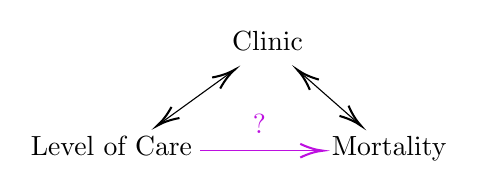
\begin{tikzpicture}[x=0.75pt,y=0.75pt,yscale=-1,xscale=1]
                  % Text Node
                  \draw (99,4) node [anchor=north west][inner sep=0.75pt]   [align=left] {Clinic};
                  % Text Node
                  \draw (2,55) node [anchor=north west][inner sep=0.75pt]   [align=left] {Level of Care};
                  % Text Node
                  \draw (147,55) node [anchor=north west][inner sep=0.75pt]   [align=left] {Mortality};
                  % Text Node
                  \draw (109,44) node [anchor=north west][inner sep=0.75pt]  [color={rgb, 255:red, 189; green, 16; blue, 224 }  ,opacity=1 ] [align=left] {?};
                  % Connection
                  \draw    (133.15,25.32) -- (160.85,49.68) ;
                  \draw [shift={(162.35,51)}, rotate = 221.32999999999998] [color={rgb, 255:red, 0; green, 0; blue, 0 }  ][line width=0.75]    (10.93,-3.29) .. controls (6.95,-1.4) and (3.31,-0.3) .. (0,0) .. controls (3.31,0.3) and (6.95,1.4) .. (10.93,3.29)   ;
                  \draw [shift={(131.65,24)}, rotate = 41.33] [color={rgb, 255:red, 0; green, 0; blue, 0 }  ][line width=0.75]    (10.93,-3.29) .. controls (6.95,-1.4) and (3.31,-0.3) .. (0,0) .. controls (3.31,0.3) and (6.95,1.4) .. (10.93,3.29)   ;
                  % Connection
                  \draw    (99.79,25.17) -- (65.71,49.83) ;
                  \draw [shift={(64.09,51)}, rotate = 324.12] [color={rgb, 255:red, 0; green, 0; blue, 0 }  ][line width=0.75]    (10.93,-3.29) .. controls (6.95,-1.4) and (3.31,-0.3) .. (0,0) .. controls (3.31,0.3) and (6.95,1.4) .. (10.93,3.29)   ;
                  \draw [shift={(101.41,24)}, rotate = 144.12] [color={rgb, 255:red, 0; green, 0; blue, 0 }  ][line width=0.75]    (10.93,-3.29) .. controls (6.95,-1.4) and (3.31,-0.3) .. (0,0) .. controls (3.31,0.3) and (6.95,1.4) .. (10.93,3.29)   ;
                  % Connection
                  \draw [color={rgb, 255:red, 189; green, 16; blue, 224 }  ,draw opacity=1 ]   (85,63) -- (142,63) ;
                  \draw [shift={(144,63)}, rotate = 180] [color={rgb, 255:red, 189; green, 16; blue, 224 }  ,draw opacity=1 ][line width=0.75]    (10.93,-3.29) .. controls (6.95,-1.4) and (3.31,-0.3) .. (0,0) .. controls (3.31,0.3) and (6.95,1.4) .. (10.93,3.29)   ;
              \end{tikzpicture}
          \end{figure}
    \item Instead of having to examine multiple $ 2\times 2 $ tables we'd like to estimate the $ \OR $
          and compute associations using a multiple regression model.
    \item One way to do this is by fitting a Binomial GLM to the data.
\end{itemize}

\makeheading{Week 4}{\daterange{2021-09-27}{2021-10-01}}
\section*{Topic 3b: Binomial Regression Models for Binary Data}
\addcontentsline{toc}{section}{Topic 3b: Binomial Regression Models for Binary Data}
\subsection*{Recall Topic 3a: Binary Data and Odds Ratios}
Last week, we introduce a simple method for association between two binary
variables, \textcolor{Blue}{$ 2\times 2 $ contingency table analysis}:
\begin{table}[!htbp]
    \centering
    \begin{NiceTabular}{l|ccc}
        & \multicolumn{2}{c}{\emph{Mortality}}                                                 \\
        Level of Care & Died                            & Survived                                 \\
        \midrule
        Intensive & $ y_1 $                            & $ m_1-y_1 $    & $ Y_1 \sim \Bin{m_1,\pi_1} $         \\
        Regular   & $ y_2 $                            & $ m_2-y_2 $    & $ Y_2 \sim \Bin{m_2,\pi_2} $      \\
        \bottomrule
    \end{NiceTabular}
\end{table}
Measure of Association: $ \displaystyle \OR = \psi=\frac{\pi_1/(1-\pi_1)}{\pi_2/(1-\pi_2)} $,
\begin{itemize}
    \item $ \OR=1 $ (equal risk).
    \item $ 0<\OR<1 $ (lower risk in group 1).
    \item $ \OR>1 $ (higher risk in group 1).
\end{itemize}
Maximum likelihood estimator for $ \OR $ is:
\[ \hat{\psi}=\frac{y_1/(m_1-y_1)}{y_2/(m_2-y_2)}, \]
and a Wald-based \qty{95}{\percent} CI is:
\[ \exp[\bigg]{\log{\hat{\psi}_1}\pm 1.96\underbrace{\sqrt{\frac{1}{y_1} +\frac{1}{m_1-y_1} +\frac{1}{y_2} +\frac{1}{m_2-y_2}}}_{\se{\log{\hat{\psi}}}}}. \]
Prenatal Care Data Example:
\begin{table}[!htbp]
    \centering
    \begin{tabular}{ccc}
        OR (\textcolor{Blue}{Mortality and Care}) & Est.                   & \qty{95}{\percent} CI             \\
        \midrule
        Intensive vs Regular                      & \textcolor{Blue}{0.51} & \textcolor{Blue}{$ (0.30,0.89) $}
    \end{tabular}
    \caption{$ 1\notin (0.30,0.89)\implies $ evidence of association between Mortality and Care.}
\end{table}
However, Mortality and Care are also related to another variable, Clinic:
\begin{table}[!htbp]
    \centering
    \begin{tabular}{ccc}
        OR (\textcolor{Blue}{Mortality and Clinic}) & Est.                   & \qty{95}{\percent} CI             \\
        \midrule
        Intensive vs Regular                        & \textcolor{Blue}{0.35} & \textcolor{Blue}{$ (0.12,0.58) $}
    \end{tabular}
    \caption{Association between Mortality and Clinic.}
\end{table}
\begin{table}[!htbp]
    \centering
    \begin{tabular}{ccc}
        OR (\textcolor{Blue}{Care and Clinic}) & Est.                    & \qty{95}{\percent} CI              \\
        \midrule
        Intensive vs Regular                   & \textcolor{Blue}{14.06} & \textcolor{Blue}{$ (9.12,21.76) $}
    \end{tabular}
    \caption{Association between Care and Clinic.}
\end{table}
\begin{itemize}
    \item Therefore, we wish to consider how a variable, e.g., Mortality ($ Y $), is related to
          multiple explanatory variables together, e.g., Care ($ x_1 $) and Clinic ($ x_2 $).
    \item This can be done using \textcolor{Blue}{multiple regression methodology} for binary data $ \implies $
          Topic 3b: Binomial Regression Models for Binary Data.
\end{itemize}
\subsection*{Multiple Regression for Binary Data}
\begin{itemize}
    \item Often we need to consider the relationship between a binary outcome and
          multiple explanatory variables, using multiple regression methodology.
    \item This is because we may want to:
          \begin{itemize}
              \item control for cofounding variables and hence want to examine the effect of
                    several variables simultaneously;
              \item examine the effect of categorical variables ($ >2 $ levels) or continuous covariates;
              \item develop sophisticated models that describe complex relationship.
          \end{itemize}
    \item Suppose \textcolor{Blue}{\emph{subject level data}} is binary with a value of 1 indicating that an event
          of interest occurs and a value of 0 indicating that event doesn't occur.
    \item Subjects can be classified according to the values of consideblue explanatory
          variables into $n$ groups (i.e., common covariates values within each group), so
          we have \textcolor{Blue}{\emph{grouped data}} such that:
          \begin{itemize}
              \item $ m_i $ denotes number of subjects in group $i$;
              \item $Y_i$ denotes number of subjects experienced the event in group $i$;
              \item $ x_{i1},\ldots,x_{ip} $ denote the covariates values associated with group $i$
                    where $ i=1,\ldots,n $.
          \end{itemize}
\end{itemize}
\subsection*{Set-up of a Binomial Regression Model}
\begin{enumerate}[label=\color{Blue}\protect\circled{\arabic*}]
    \item \textcolor{Blue}{Response Variable}: $ Y_i \sim \Bin{m_i,\pi_i} $, $ i=1,\ldots,n $, and Binomial
          distribution is a member of Exponential family!
          \begin{align*}
              f(y_i)
               & =\binom{m_i}{y_i}\pi_i^{y_i}(1-\pi_i)^{m_i-y_i}                                   \\
               & =\exp*{y_i\log*{\frac{\pi_i}{1-\pi_i}}+m_i\log{1-\pi_i}+\log*{\binom{m_i}{y_i}}},
          \end{align*}
          where
          \begin{align*}
              \theta_i     & =\log*{\frac{\pi_i}{1-\pi_i}},              \\
              a(\phi)=\phi & =1,                                         \\
              b(\theta_i)  & =-m_i\log{1-\pi_i}=m_i\log{1+e^{\theta_i}}. \\
              c(y_i;\phi)  & =\log*{\binom{m_i}{y_i}}.
          \end{align*}
    \item \textcolor{Blue}{Linear Predictor}:
          \[ \eta_i=\Vector{x}_i^\top \Vector{\beta}=\beta_0+\beta_1x_{i1}+\cdots+\beta_p x_{ip}. \]
    \item \textcolor{Blue}{Link Function}: Recall that for Binomial distribution, we have $ \E{Y_i}=\mu_i=m_i\pi_i $,
          therefore we typically re-write the link function in terms of $ \pi_i $,
          \[ \textcolor{Blue}{g(\pi_i)}=\Vector{x}_i^\top \Vector{\beta}. \]
          As $ \pi_i\in(0,1) $, any function $ g\colon (0,1)\to(-\infty,\infty) $ may work, and here are some link functions we
          can consider:
          \begin{table}[!htbp]
              \centering
              \begin{tabular}{cc}
                  \toprule
                  log-log                             & $ g(\pi)=\log[\big]{-\log{\pi}} $                                               \\
                  complementary log-log               & $ g(\pi)=\log[\big]{-\log{1-\pi}} $                                             \\
                  Probit$^a$                          & $ g(\pi)=\Phi^{-1}(\pi) $                                                       \\
                  Logit (\textcolor{Blue}{canonical}) & $ g(\pi)=\log[\big]{\pi/(1-\pi)} $                                              \\
                  \bottomrule
                  \multicolumn{2}{l}{\footnotesize{$ {}^a $For the Probit link, $ \Phi(\:\cdot\:) $ is the \emph{CDF} of $ \N{0,1} $.}} \\
              \end{tabular}
          \end{table}
\end{enumerate}
\subsection*{Canonical Link and Logistic Regression}
Recall for Binomial distribution
\end{document}
